\documentclass{article}

\usepackage{geometry}
\geometry{a4paper}
\setlength{\parindent}{10mm}
\setlength{\parskip}{0.9em}
\def\baselinestretch{1.5}

\usepackage[spanish,mexico]{babel}
\renewcommand {\spanishtablename}{Cuadro}
\usepackage[spanish,onelanguage,ruled]{algorithm2e}
\usepackage[utf8]{inputenc}
\usepackage{graphicx}
\usepackage{caption} 
\usepackage{amsmath, amsthm, amsfonts}
\usepackage{enumerate} 
\usepackage{fancyhdr}
\usepackage{anysize} 
\usepackage[usenames]{color}
\usepackage{booktabs}
\usepackage{etoolbox}
\usepackage{fancyvrb}
\usepackage{color,soul}
\usepackage[dvipsnames]{xcolor}
\usepackage{graphicx}
 \usepackage{caption}
\usepackage{subcaption}
\usepackage{listings}
\usepackage{amssymb}
\usepackage{multirow}



\usepackage{verbatim}
% redefine \VerbatimInput
\RecustomVerbatimCommand{\VerbatimInput}{VerbatimInput}%
 {fontsize=\footnotesize,
  %
  frame=lines,  % top and bottom rule only
  framesep=1em, % separation between frame and text
  rulecolor=\color{Gray},
  %
  label=\fbox{\color{Black}test.txt},
  labelposition=topline,
  %
  %commandchars=\ \mid \(\), % escape character and argument delimiters for
                  % commands within the verbatim
  %commentchar=*        % comment character
 }


\pagestyle{fancy}

\chead{}
\lhead{} 
\rhead{}
\lfoot{\it }
\cfoot{}
\rfoot{\thepage}

\title{
\centering
Modelos Probabilistas Aplicados \\
Johanna Bolaños Zúñiga \\
Matricula: 1883900\\
Tarea 10
}

\date{}

\begin{document}
\maketitle

\section{Simulación de problemas}
En el presente trabajo se realizaron algunas simulaciones para comparar los resultados analíticos de las soluciones de diversos problemas del libro de Grinstead \cite{librop} sobre el valor esperado, varianza y desviación estándar de una variable aleatoria (v.a) discreta y continua. Para el cálculo de estos valores se utilizaron las ecuaciones \ref{discreta}, \ref{continua}, \ref{varianza} y \ref{desviacion}, donde $X$ es una v.a con espacio muestral $\Omega$ y distribución de probabilidad $f{(x)}$:

\noindent Valor esperado si $X$ es discreta 
\begin{equation}
\mu = E{(X)} = \sum_{x \in \Omega}xf(x).
\label{discreta}
\end{equation}
\noindent Valor esperado si $X$ es continua,
\begin{equation}
\mu = E{(X)} = \int_{-\infty}^{\infty}xf(x)dx.
\label{continua}
\end{equation}
\noindent Varianza de $X$,
\begin{equation}
\sigma^2 = V(X)= E{(X^2)} - \mu^2.
\label{varianza}
\end{equation}
\noindent Desviación estándar de $X$,
\begin{equation}
\sigma = D(X)= \sqrt{V(X)}.
\label{desviacion}
\end{equation}

Todas las simulaciones fueron realizadas en el software R versión 4.0.2 \cite{r} y el código empleado se encuentra en el repositorio GitHub \cite{github}.

\subsection{Problema $1$, página $247$} \label{problema1}
\textit{A card is drawn at random from a deck consisting of cards numbered $2$ through $10$. A player wins 1 dollar if the number on the card is odd and loses $1$ dollar if the number if even. What is the expected value of his winnings?}

\noindent \textbf{Solución}

Cantidad total de cartas = $9$, donde hay $5$ cartas pares y $4$ impares. Si se saca una carta par, se pierde $1$ dólar, de lo contrario, se gana $1$ dólar. Entonces, sea $X$ el evento de que la carta sacada sea par o impar. El valor esperado de ganancia fue calculado mediante la ecuación \ref{discreta} dando como resultado un $E{(X)}$ = $-\frac{1}{9} \thickapprox -0.11$.

Con el fin de identificar si este juego es desfavorable con un $E{(x)} \thickapprox -0.11$,  se utilizó la función \texttt{sample()} para para realizar una simulación donde se saca $1$ carta en la primera jugada, luego $2$ cartas en la segunda jugada y así sucesivamente hasta llegar a $100$ jugadas (es decir, se sacan $100$ cartas), se calcula el valor esperado en cada jugada y se contabilizó la frecuencia de estos valores. 

En la figura \ref{cartasa}, se muestran los resultados obtenidos de esta simulación, en la que podemos observar que, de las $100$ jugadas, la mayoría de veces ($79$ jugadas) este no es un juego favorable y en promedio el valor esperados más frecuentes es $-0.1$. De igual forma, se realizó la simulación desde $1$ hasta $1,000$ jugadas (ver figura \ref{cartasb}) y el resultado fue el mismo, en la mayoría de veces ($960$ jugadas) arrojó un valor esperado negativo, siendo en promedio el más frecuentes de $-0.1$. Por lo anterior, se concluye que tanto analíticamente como experimentalmente, el juego de las cartas descrito en el problema \ref{problema1}, es un juego desfavorable.

\begin{figure}[h]
    \begin{center}
    \captionsetup{justification=centering}
    \begin{subfigure}[b]{0.45\textwidth}
        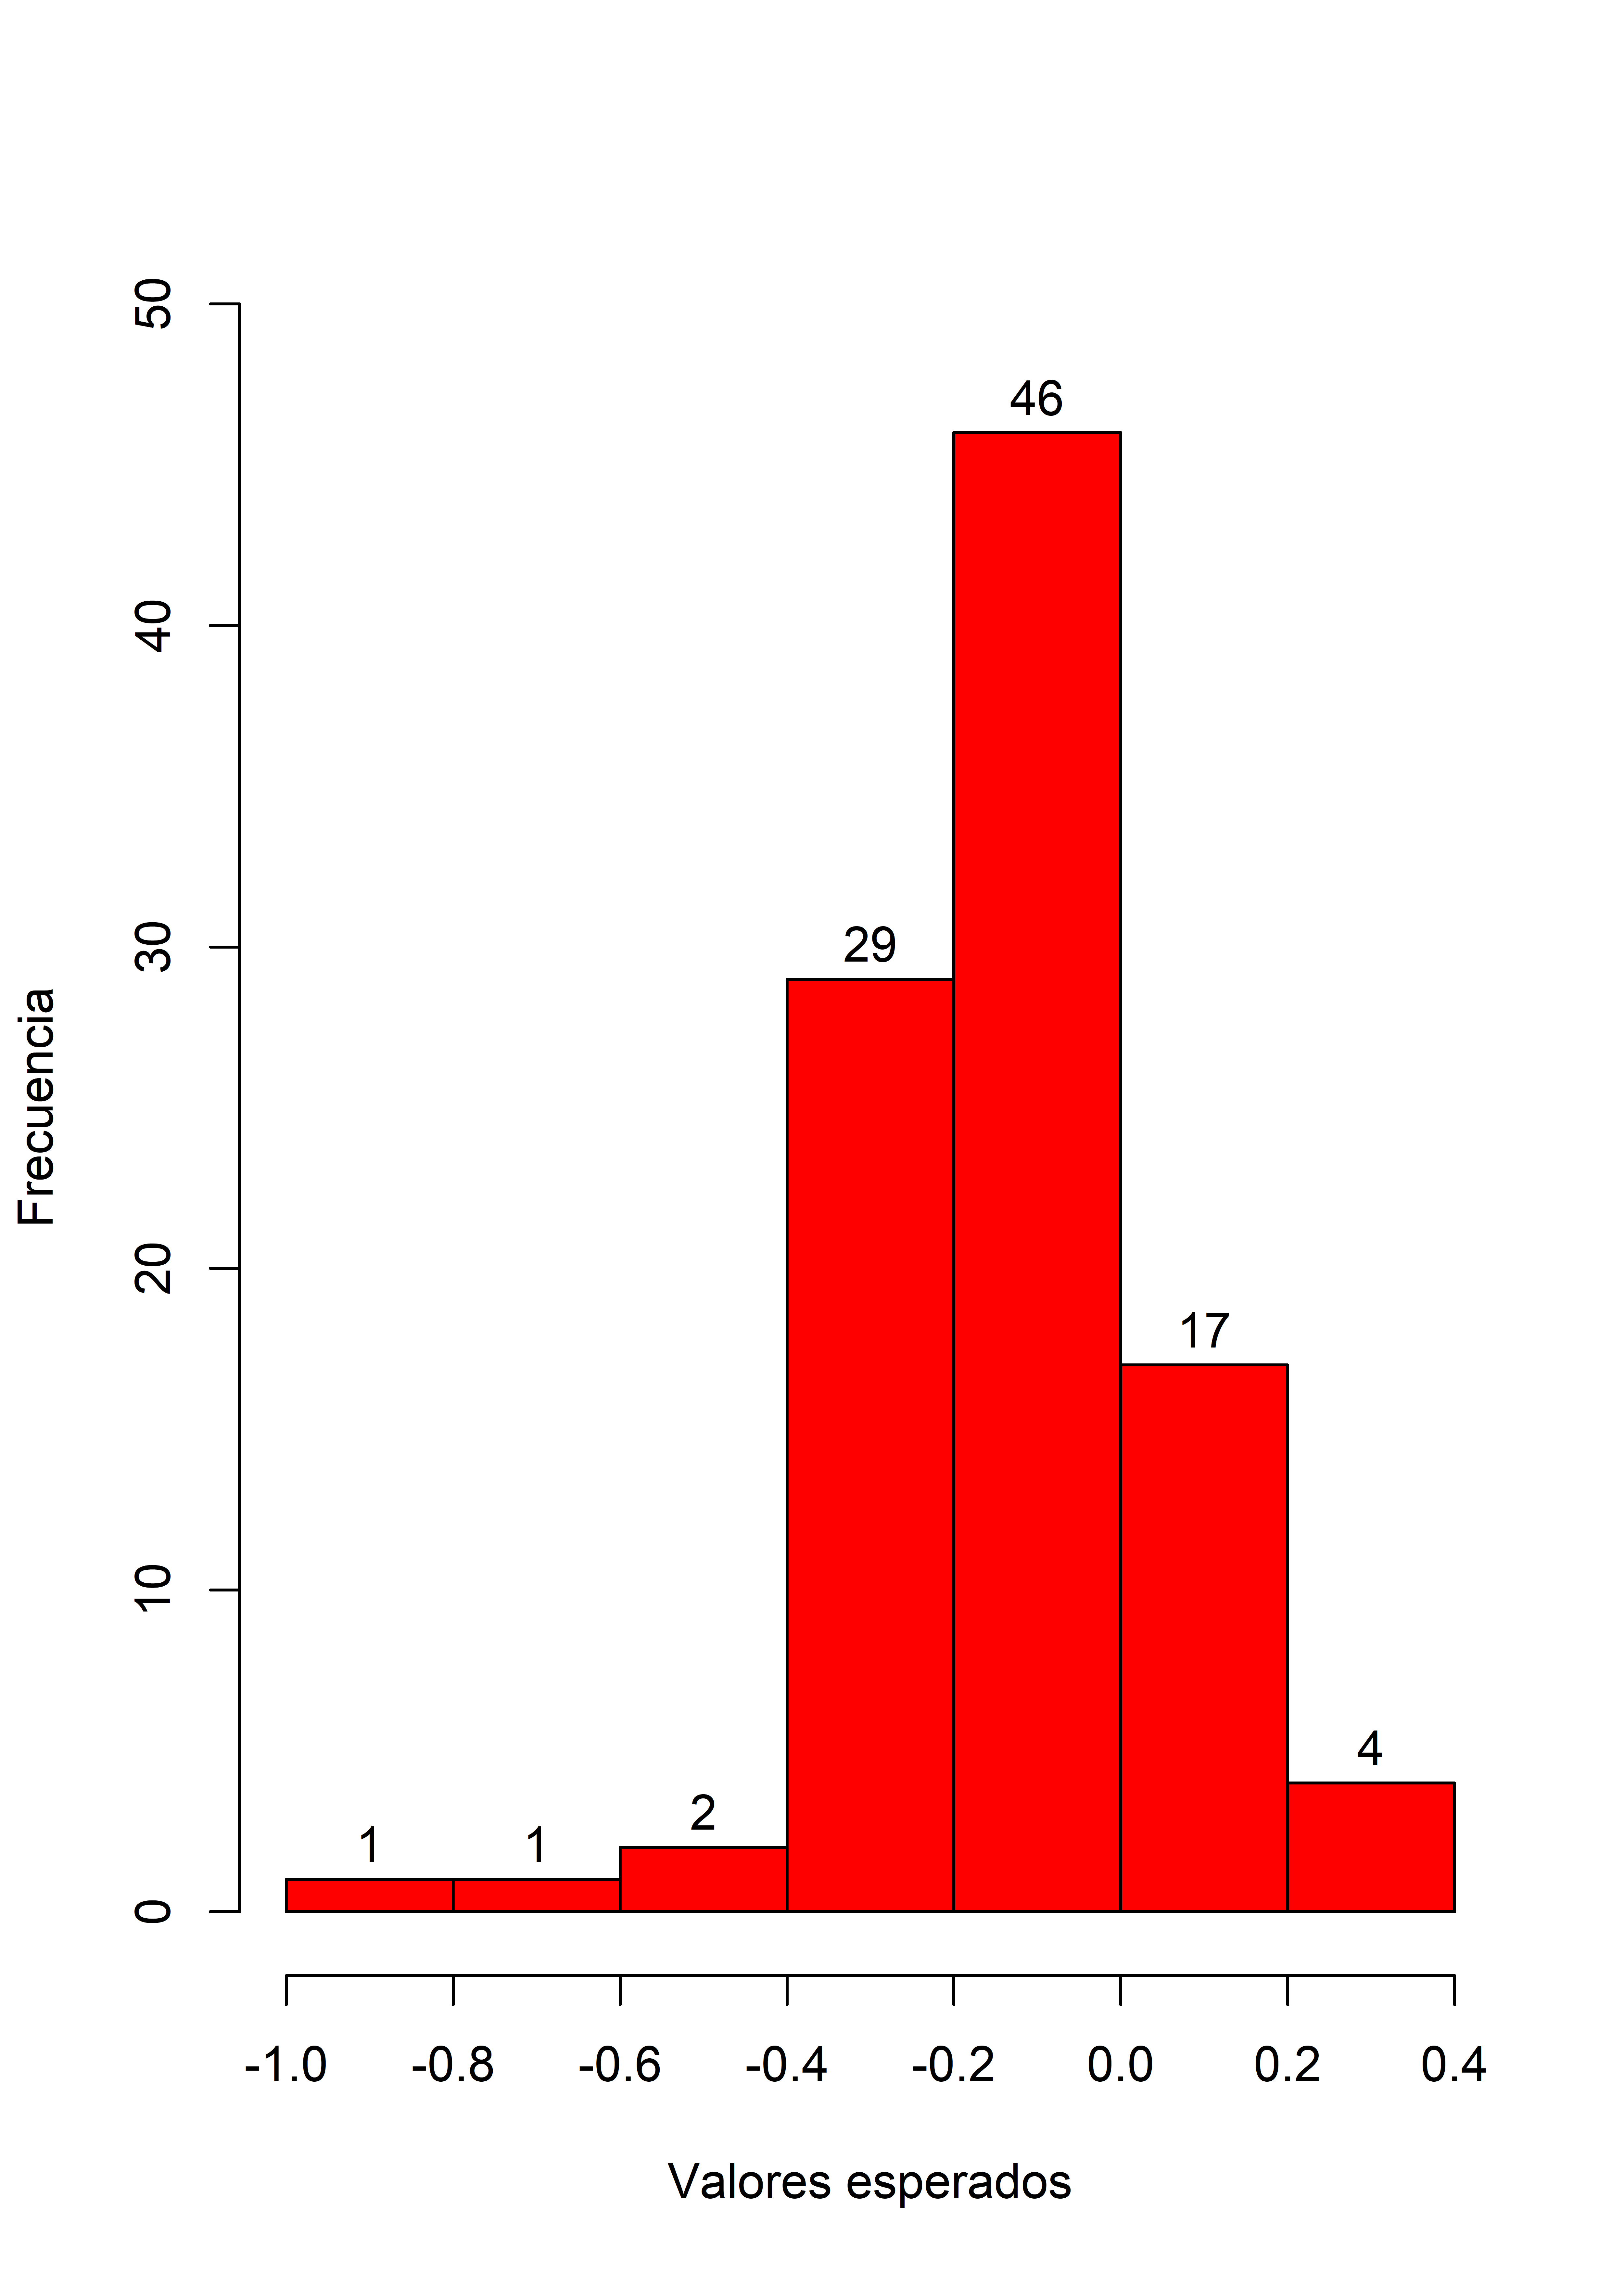
\includegraphics[scale=0.5]{Figures/cartas100.png}
        \caption{Desde $1$ hasta $100$ jugadas}
        \label{cartasa}
    \end{subfigure}
    \begin{subfigure}[b]{0.5\textwidth}
        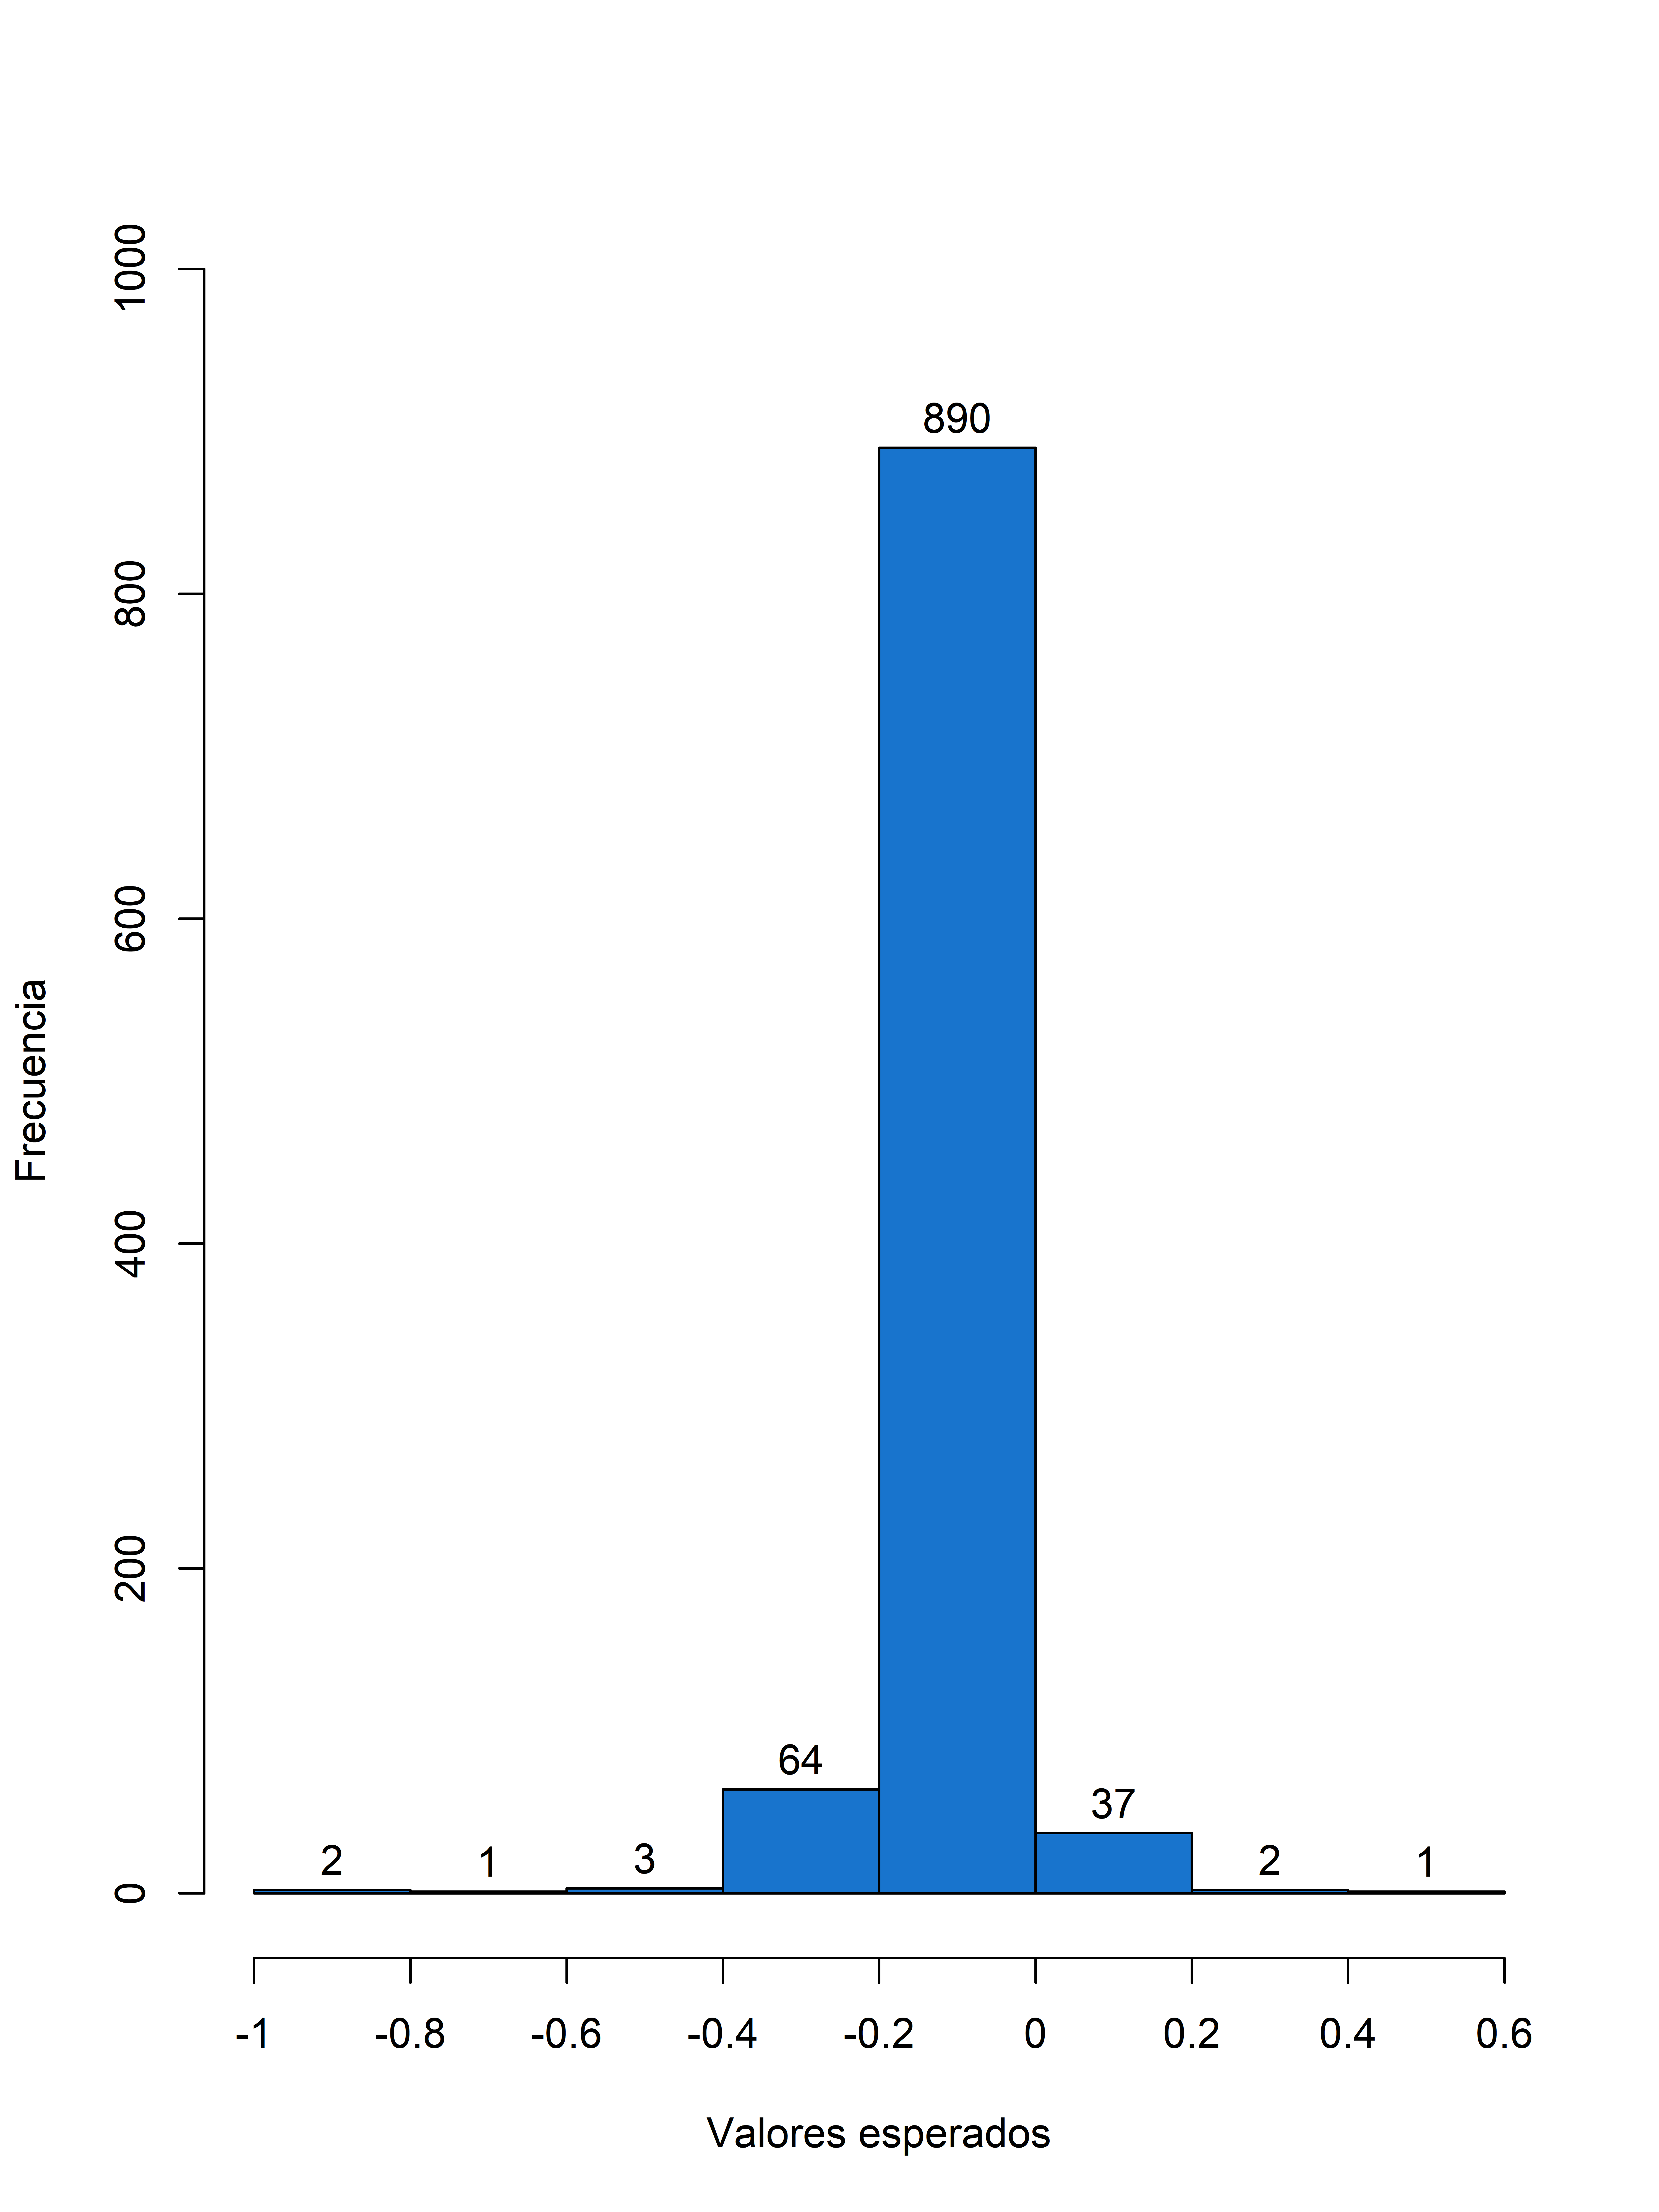
\includegraphics[scale=0.45]{Figures/cartas1000.png}
        \caption{Desde $1$ hasta $1,000$ jugadas}
        \label{cartasb}
    \end{subfigure}
    \caption{Resultados simulación del valor esperado para el problema \ref{problema1}}
    \label{cartas}
    \end{center}
\end{figure}

\subsection{Problema $9$, página $264$} \label{problema2}
\textit{A die is loaded so that the probability of a face coming up is proportional to the number on that face. The die is rolled with outcome $X$. Find $V(X)$ and $D(X)$.}

\noindent \textbf{Solución}

Se tiene que la probabilidad de cada cara de este dado cargado es de $p{(x)} = \frac{x}{21}$. El valor esperado, la varianza y desviación estándar fueron calculados mediante las ecuaciones \ref{discreta}, \ref{varianza} y \ref{desviacion}, respectivamente, las cuales arrojaron como resultado que el $E{(X)}$ = $\frac{13}{3} \thickapprox 4.33$, la $V{(X)}$ = $\frac{20}{9} \thickapprox 2.22$ y una $D{(X)} \thickapprox 1.49$.

Se realizó una simulación para comparar si el valor esperado, varianza y desviación estándar calculados anteriormente, es el mismo para $n$ lanzamientos. Se utilizó la función \texttt{sample()} para generar conjuntos con $10$, $11$, $12$ y así sucesivamente, hasta de $100$ lanzamientos, se calculó el valor esperado, varianza y desviación estándar correspondiente en cada conjunto y se contabilizó la frecuencia de estos valores. Los resultados de esta simulación se muestran en la figura \ref{dados}. 
%width=.99\linewidth
\begin{figure}[htp]
    \begin{center}
    \captionsetup{justification=centering}
    \centering
    \begin{subfigure}{0.45\textwidth}
        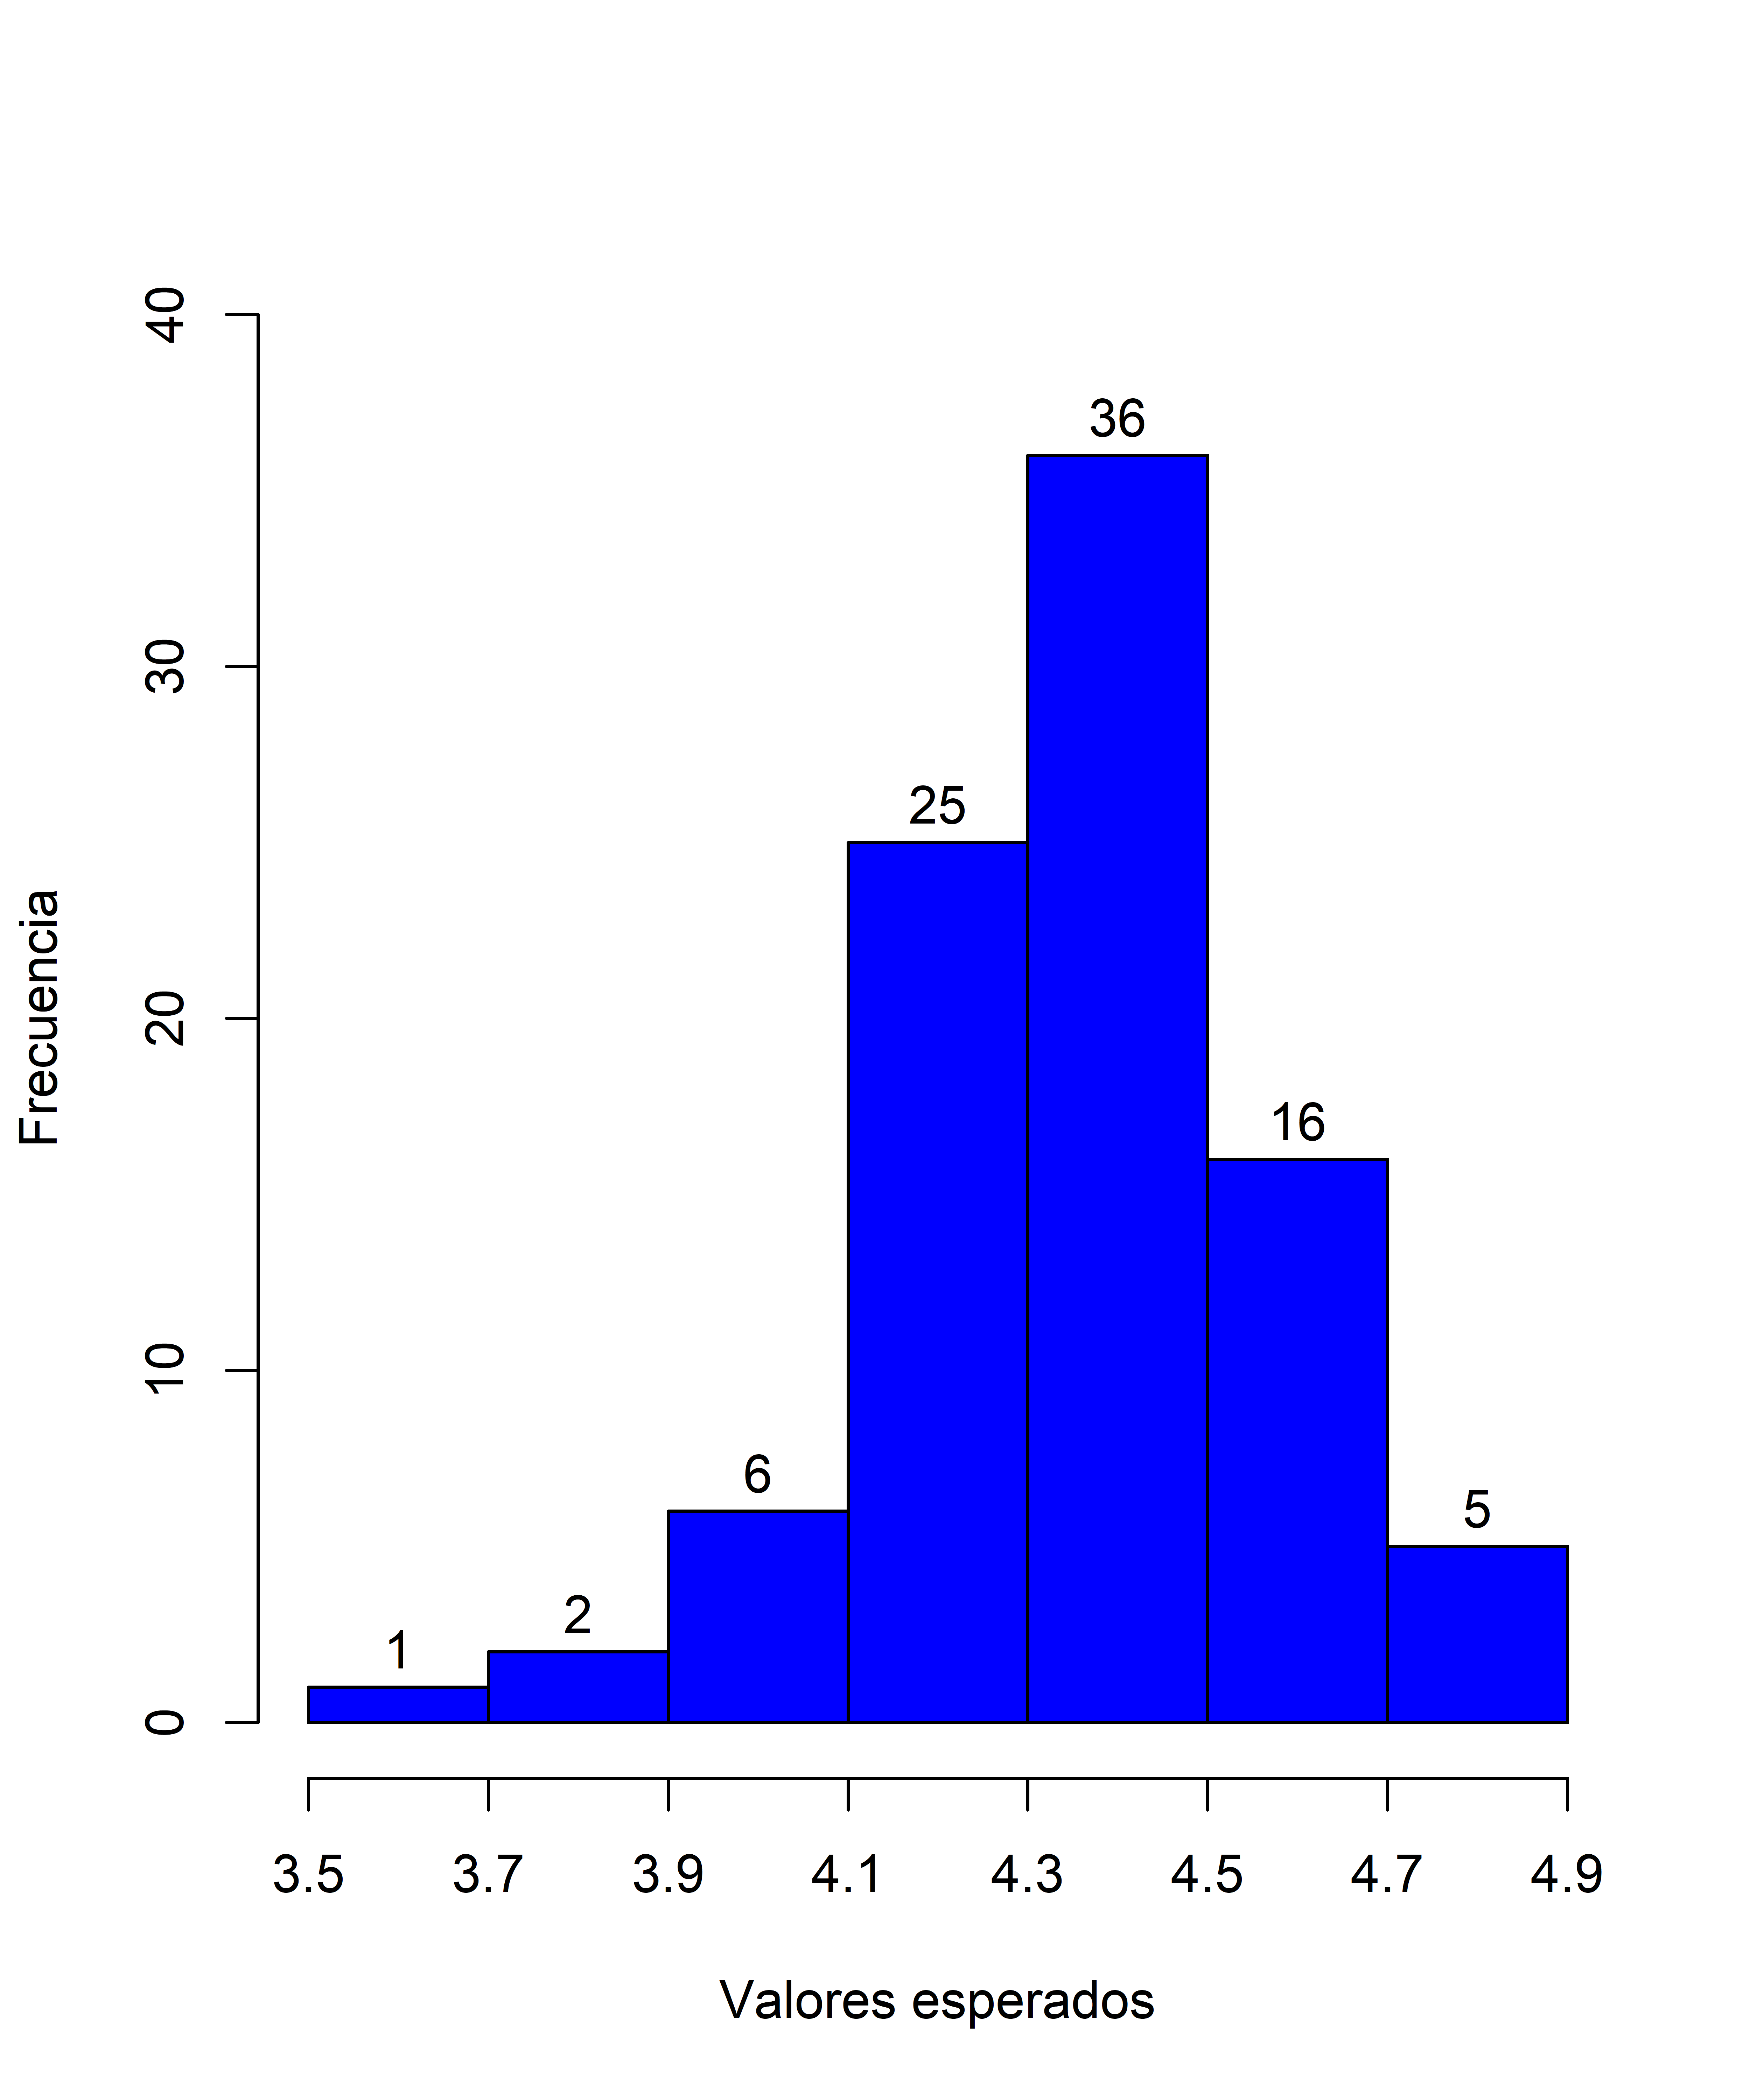
\includegraphics[scale=0.55]{Figures/dadosVE.png}
        \caption{Valores esperados}
        \label{dadosVE}
    \end{subfigure}
    \begin{subfigure}{0.45\textwidth}
        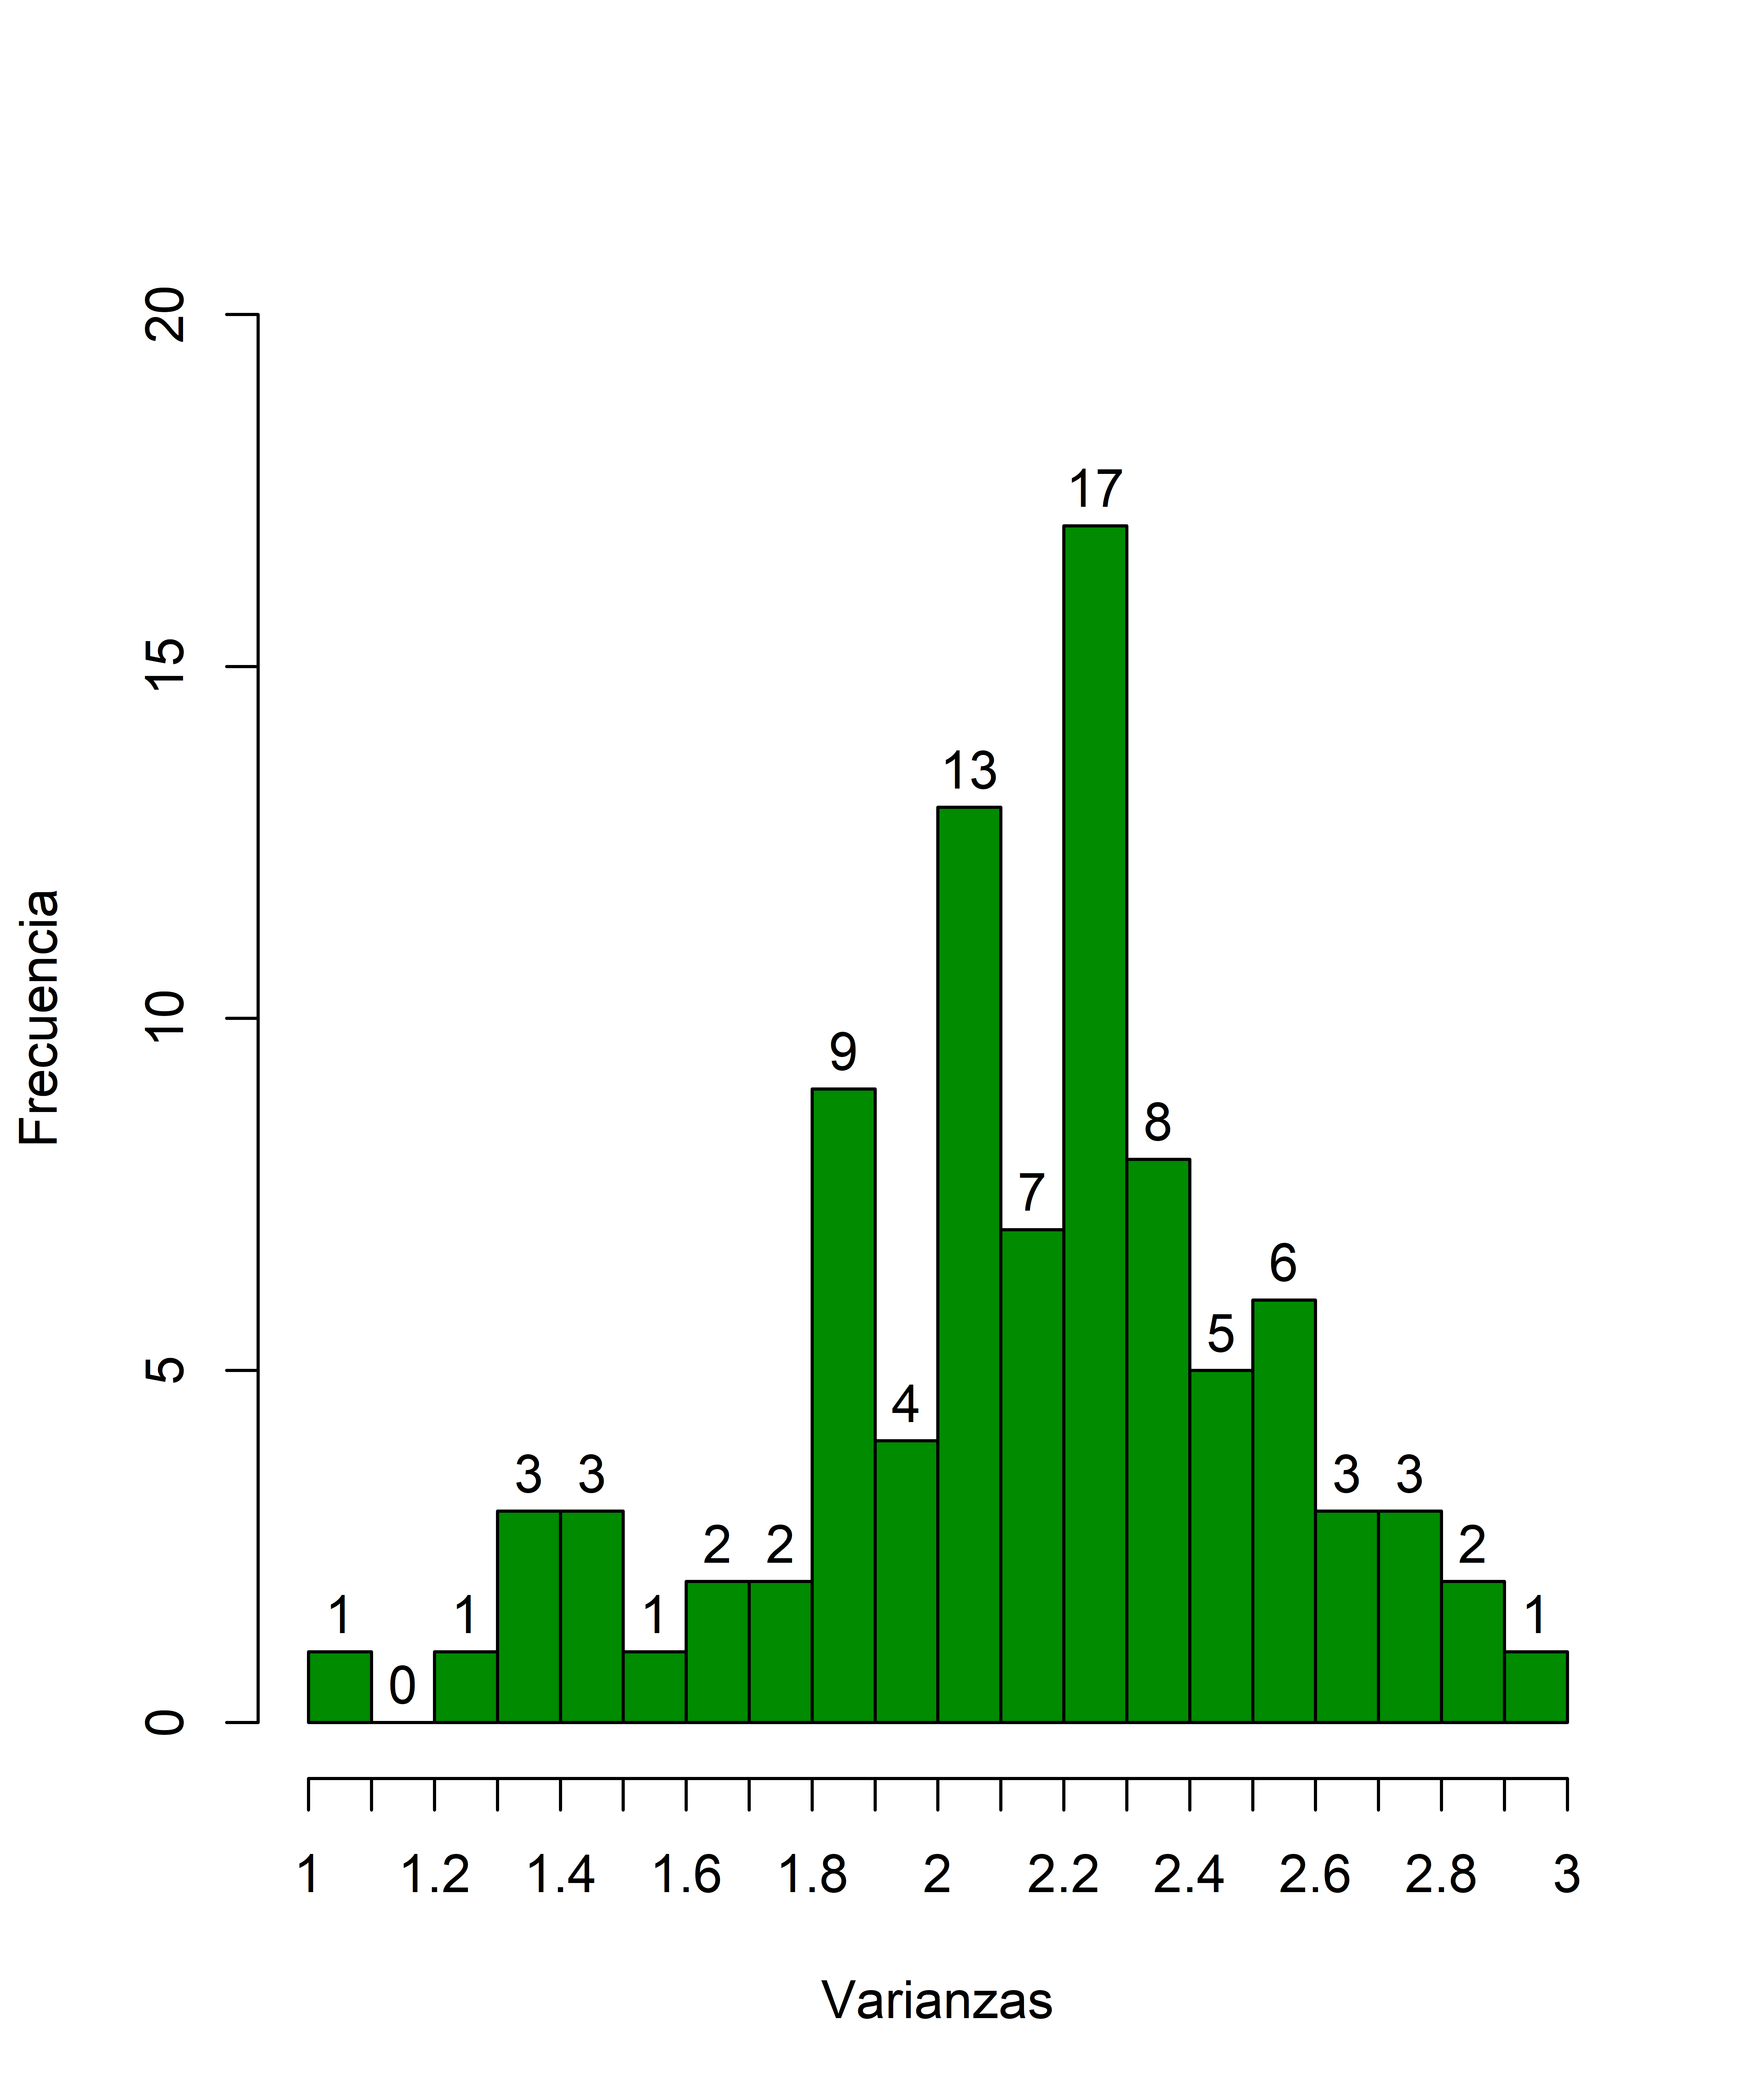
\includegraphics[scale=0.55]{Figures/dadosVar.png}
        \caption{Varianzas}
        \label{dadosVar}
    \end{subfigure}
    \begin{subfigure}{0.45\textwidth}
        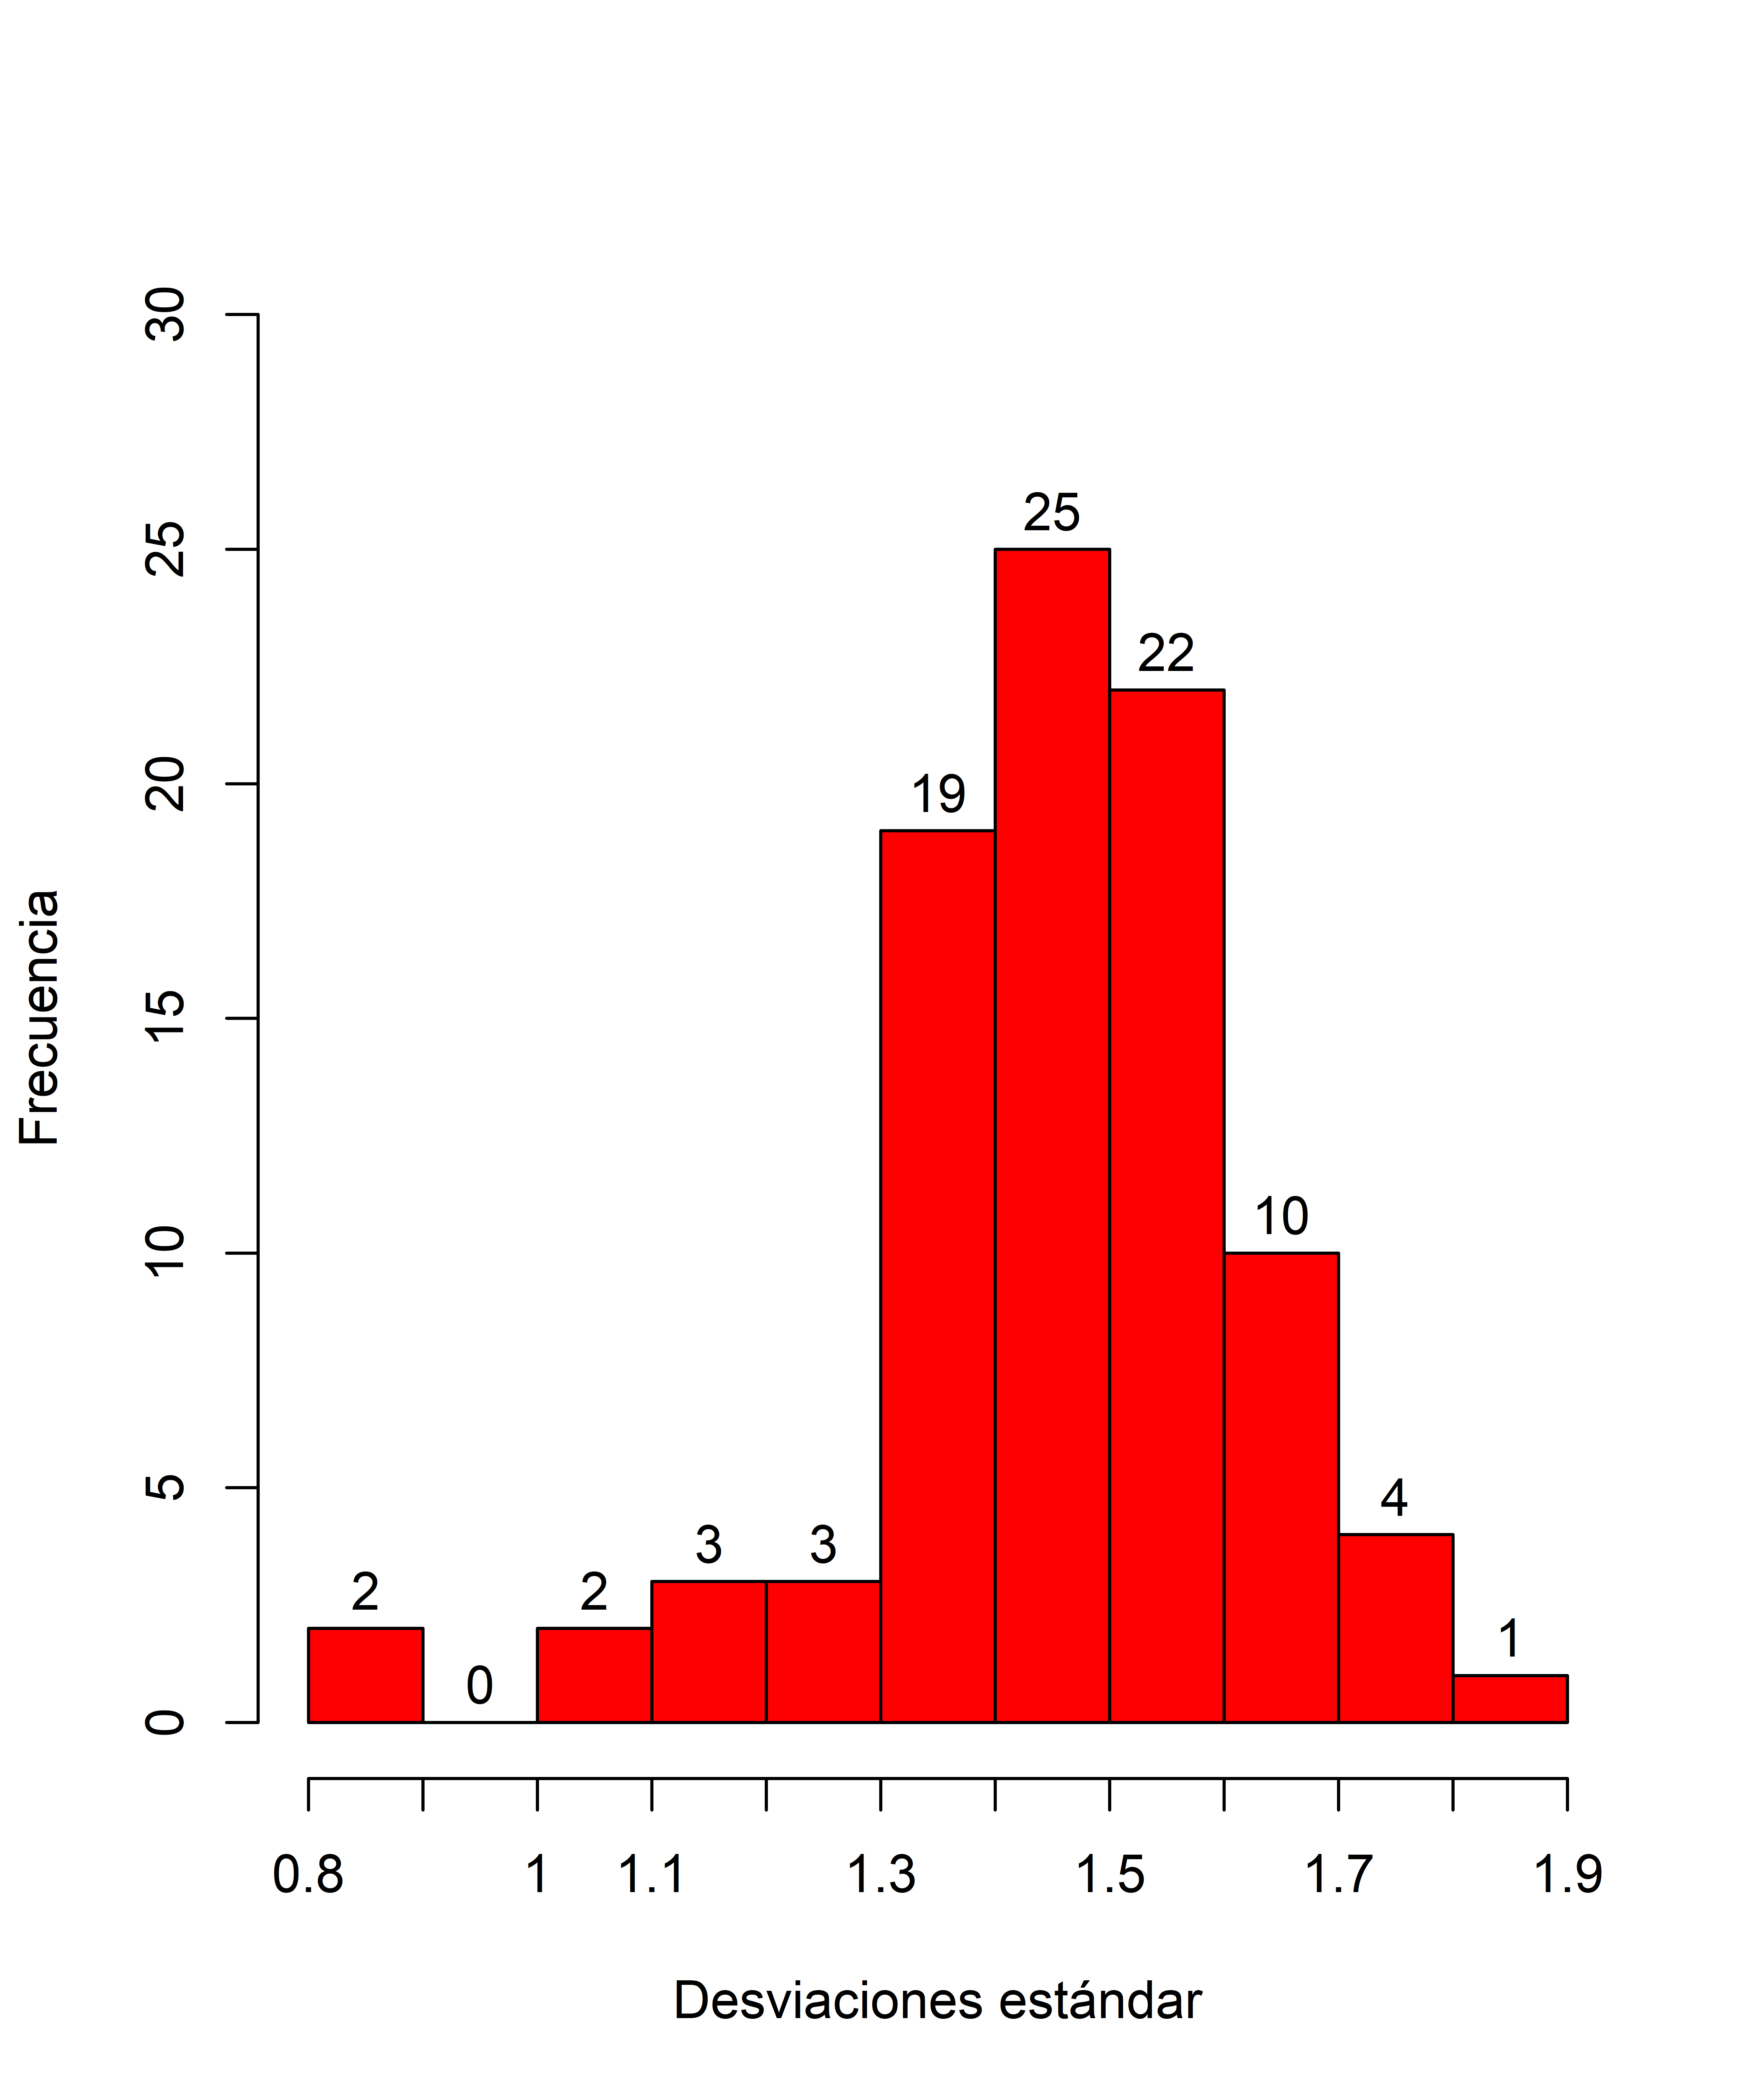
\includegraphics[scale=0.55]{Figures/dadosDesv.png}
        \caption{Desviaciones estándar}
        \label{dadosDesv}
    \end{subfigure}
    \caption{Resultados de la simulación del problema \ref{problema2}}
    \label{dados}
    \end{center}
\end{figure}

En la figura \ref{dadosVE}, podemos observar que de los 91 conjuntos de lanzamientos el valor esperado más frecuente es, aproximadamente, de $4.3$, en la figura \ref{dadosVar}, el valor de la varianza más frecuente está alrededor de $2.2$ y en la figura \ref{dadosDesv} el valor de la desviación estándar más frecuente en promedio es de $1.45$. Por lo anterior, se puede concluir que tanto analíticamente como experimentalmente, en este dado cargado las caras con mayor probabilidad de salir son la $4$, $5$ y $6$ con una desviación estándar de, aproximadamente, $1.45$ como se puede observar en la figura \ref{dados1}.

\begin{figure}[h]
    \begin{center}
    \captionsetup{justification=centering}
    \begin{subfigure}{0.32\textwidth}
        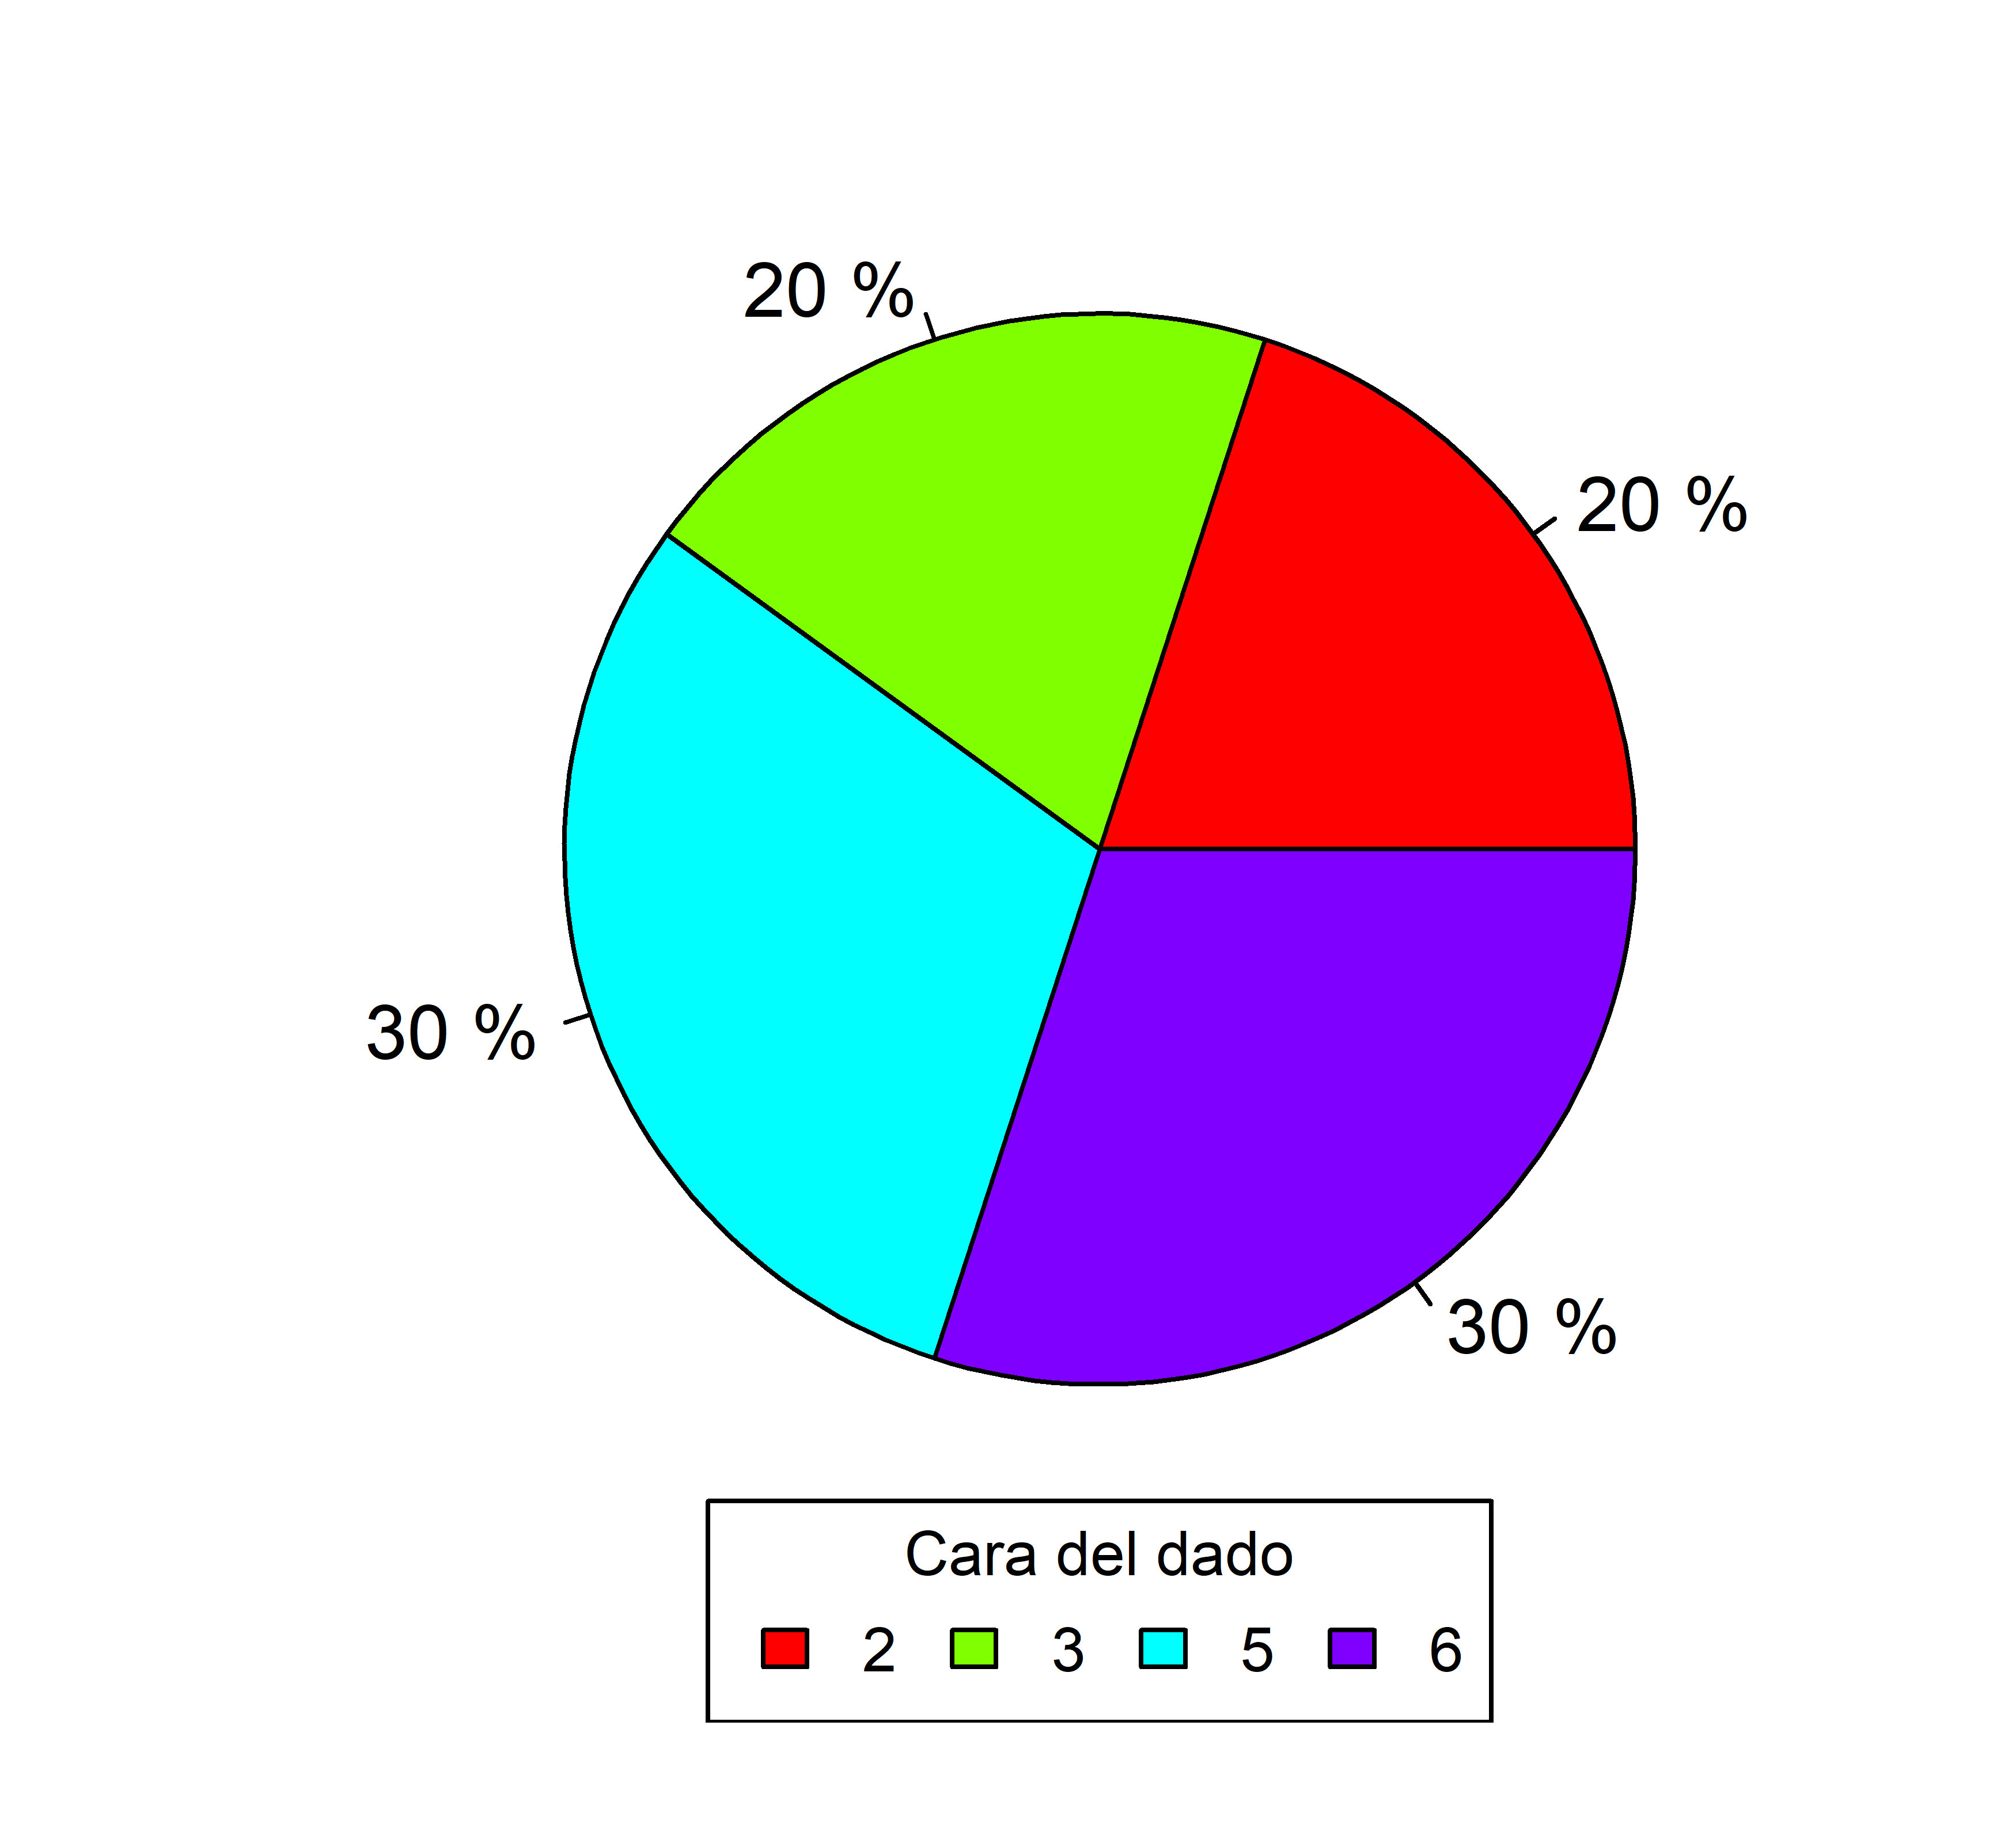
\includegraphics[width=.99\linewidth]{Figures/dados10-.png}
        \caption{En $10$ lanzamientos}
    \end{subfigure}
    \begin{subfigure}{0.32\textwidth}
        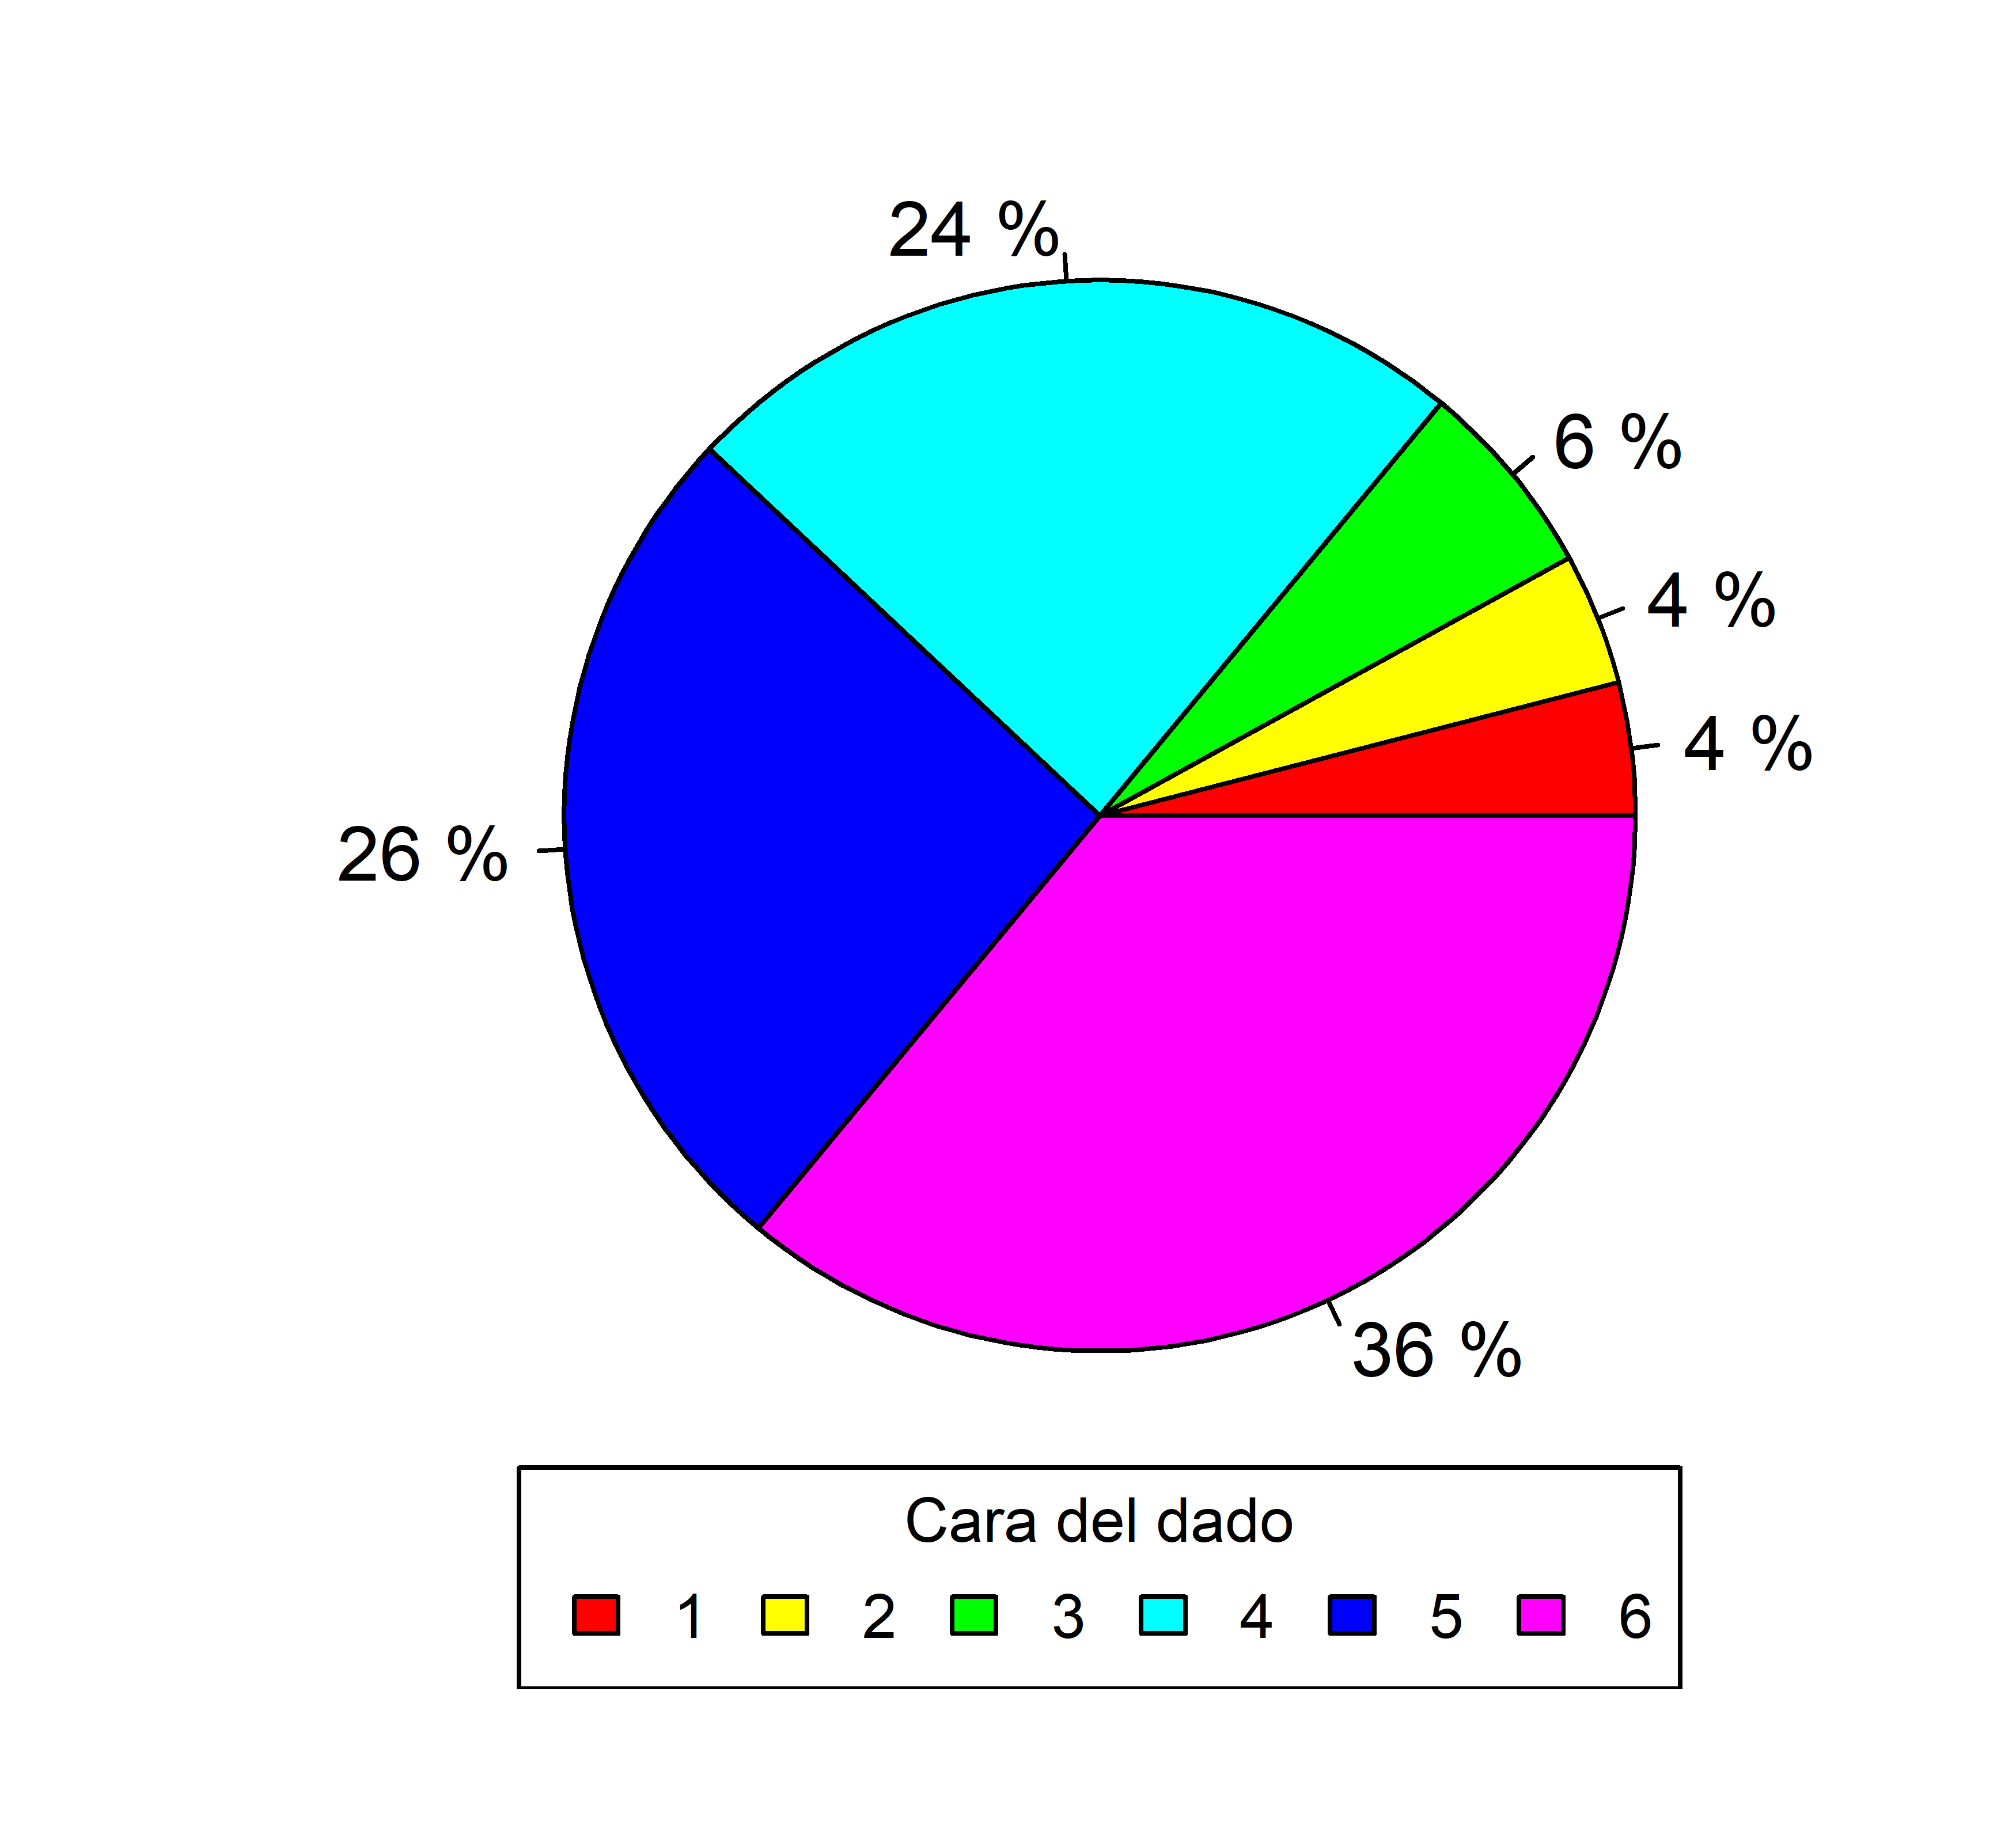
\includegraphics[width=.99\linewidth]{Figures/dados50-.png}
        \caption{En $50$ lanzamientos}
    \end{subfigure}
    \begin{subfigure}{0.32\textwidth}
        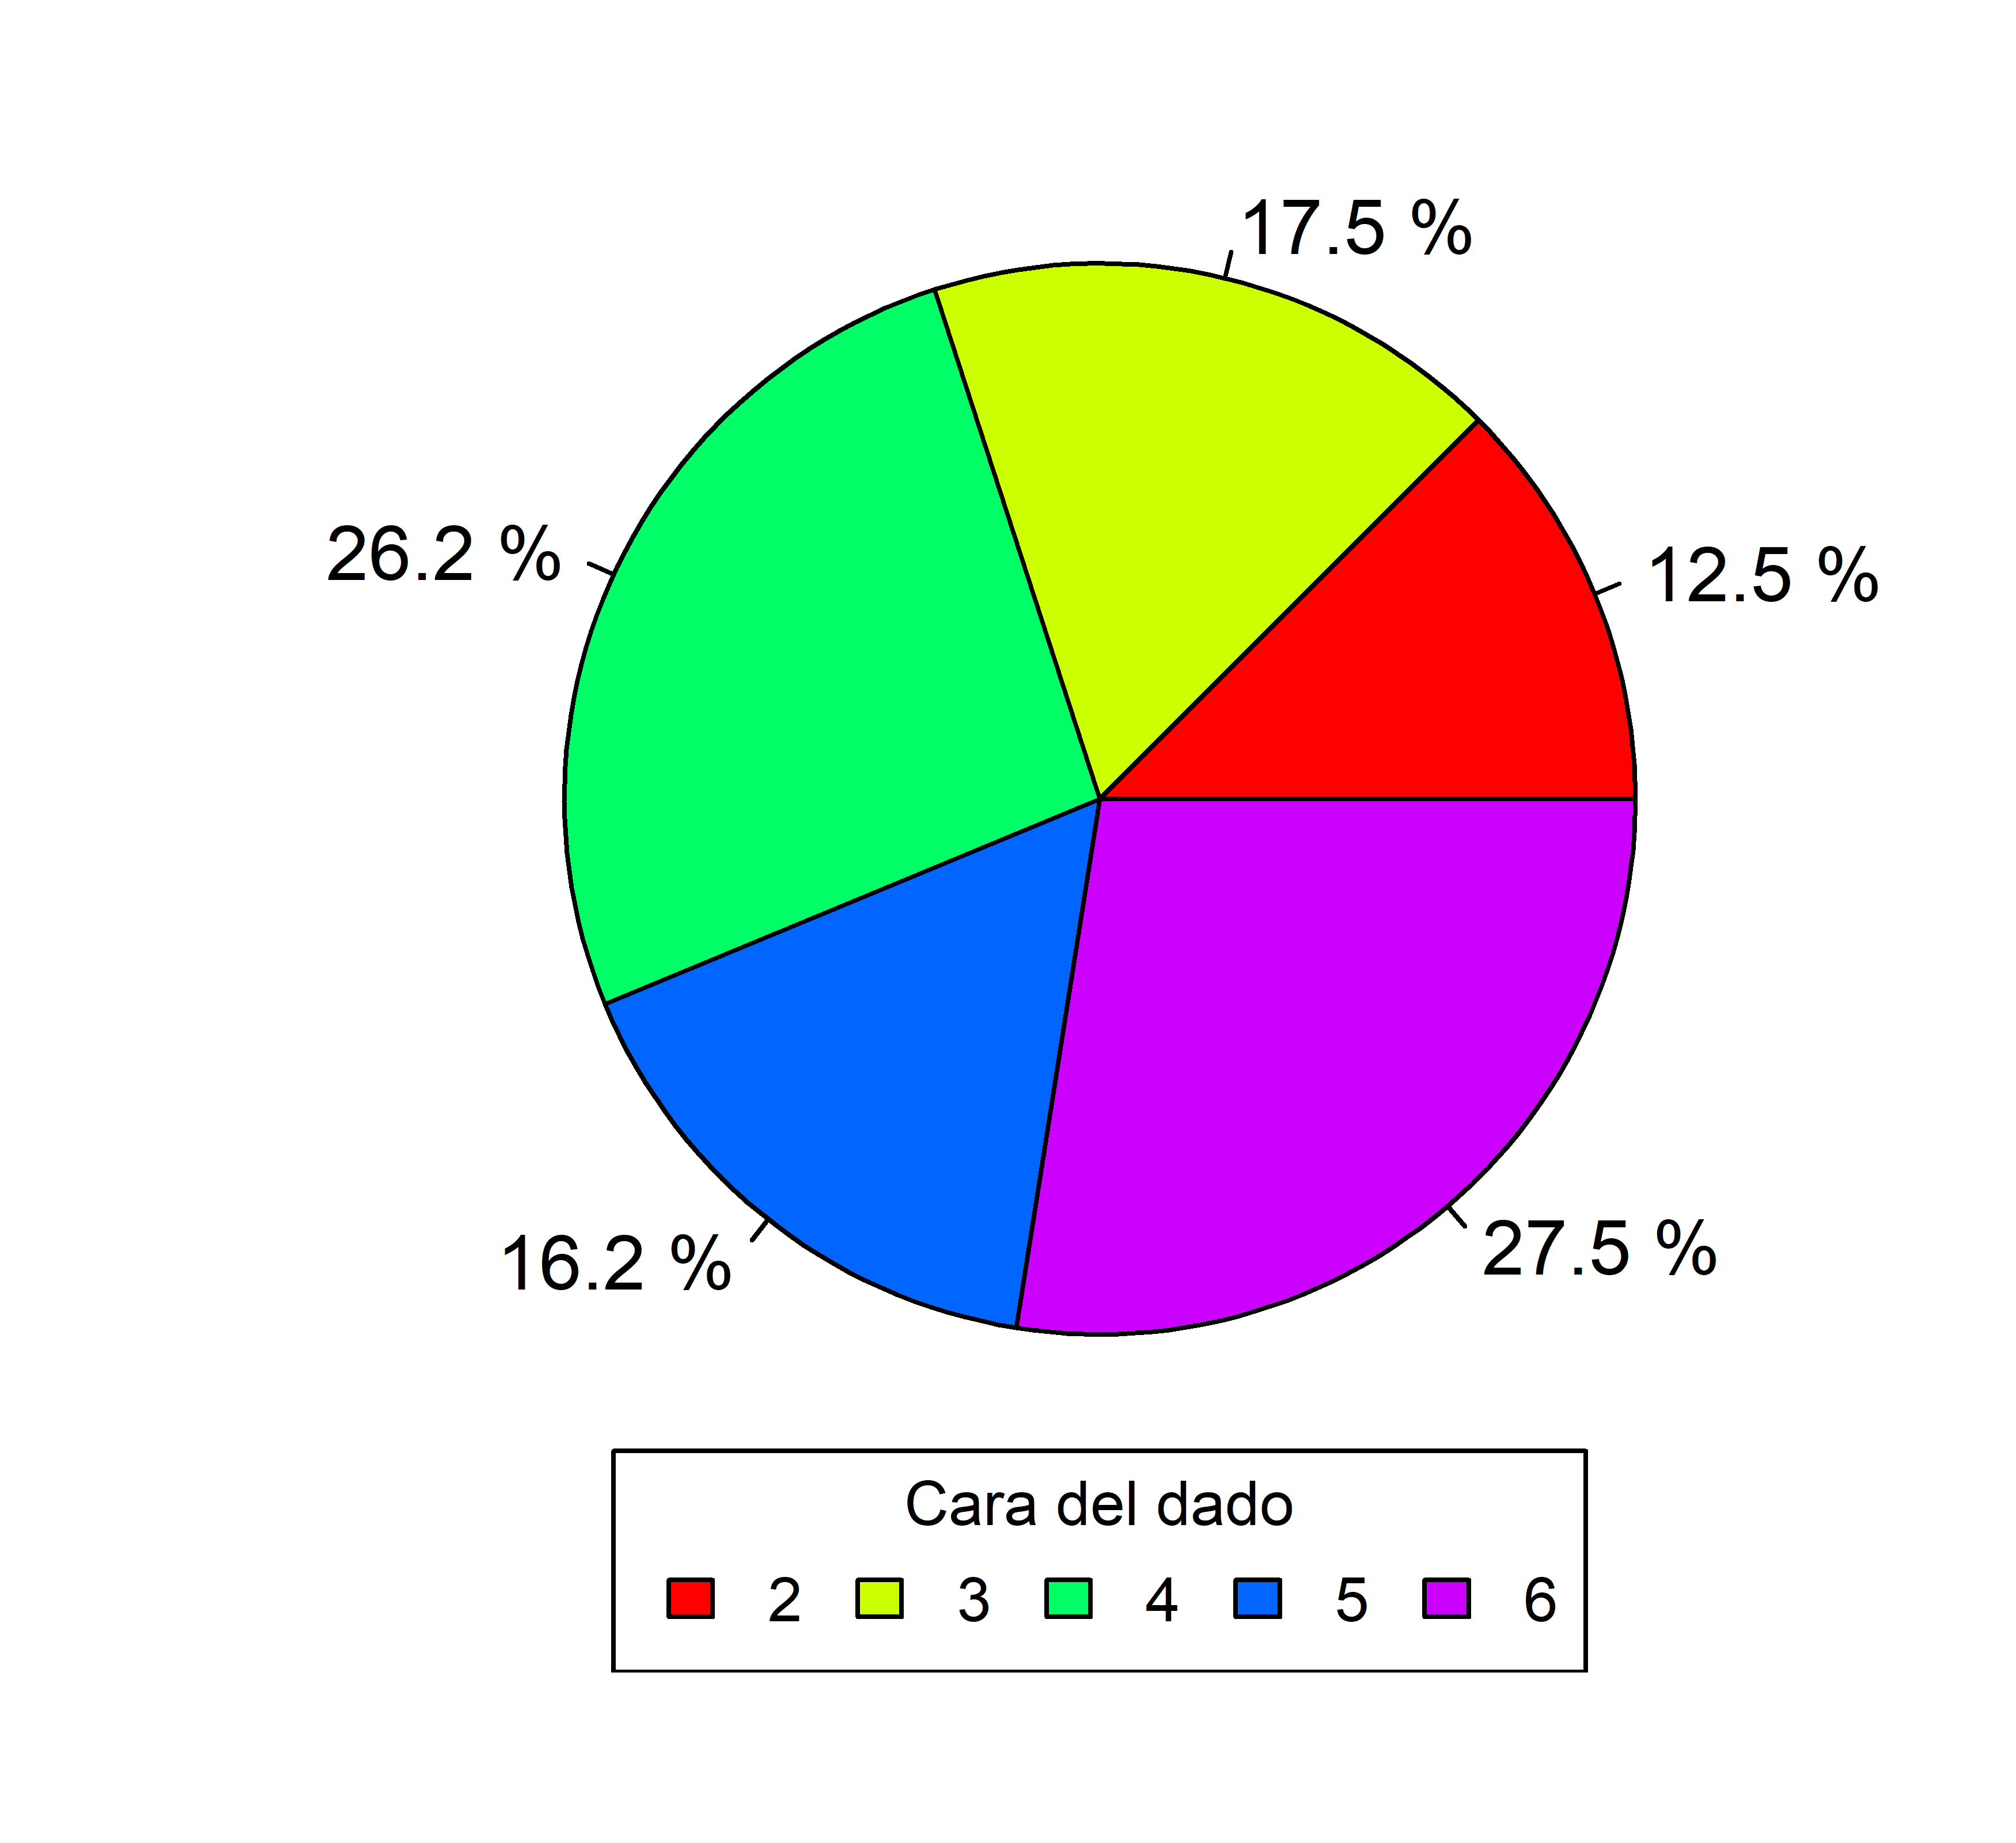
\includegraphics[width=.99\linewidth]{Figures/dados80-.png}
        \caption{En $80$ lanzamientos}
    \end{subfigure}
    \caption{Resultado de la frecuencia de ocurrencias de las caras del dado cargado del problema \ref{problema2}}
    \label{dados1}
    \end{center}
\end{figure}

\subsection{Problema 1, página 263} \label{problema4}
\texttt{A number is chosen at random from the set $S$ = \{$-1, 0, 1$\}. Let $X$ be the number chosen. Find the expected value, variance, and standard deviation of $X$.}

\noindent \textbf{Solución}

\noindent Sea $X$ el número escogido, por lo tanto, $p(x)$ = $1/3$, el valor esperado de $X$, la varianza y desviación estándar fueron calculados mediante las ecuaciones \ref{discreta}, \ref{varianza} y \ref{desviacion}, las cuales dieron como resultado un $E{(X)}$ = $0$, una $V{(X)}$ = $\frac{2}{3} \thickapprox 0.66$ y una $D{(X)}$ $\thickapprox 0.816$.

Para este problema, en la simulación se consideró realizar $10,000$ selecciones entre los números $-1$, $0$ y $1$ y se calculó el valor esperado, varianza y desviación estándar con los datos obtenidos. Como resultado de esta simulación se obtuvo un valor esperado de $-0.002$, una varianza de $0.670$ y una desviación estándar de $0.818$, lo cual es muy similar a los valores obtenidos de manera analítica. En la figura \ref{seleccion} se muestra la frecuencia de selección de $X$.


\begin{figure}[h]
\centering
    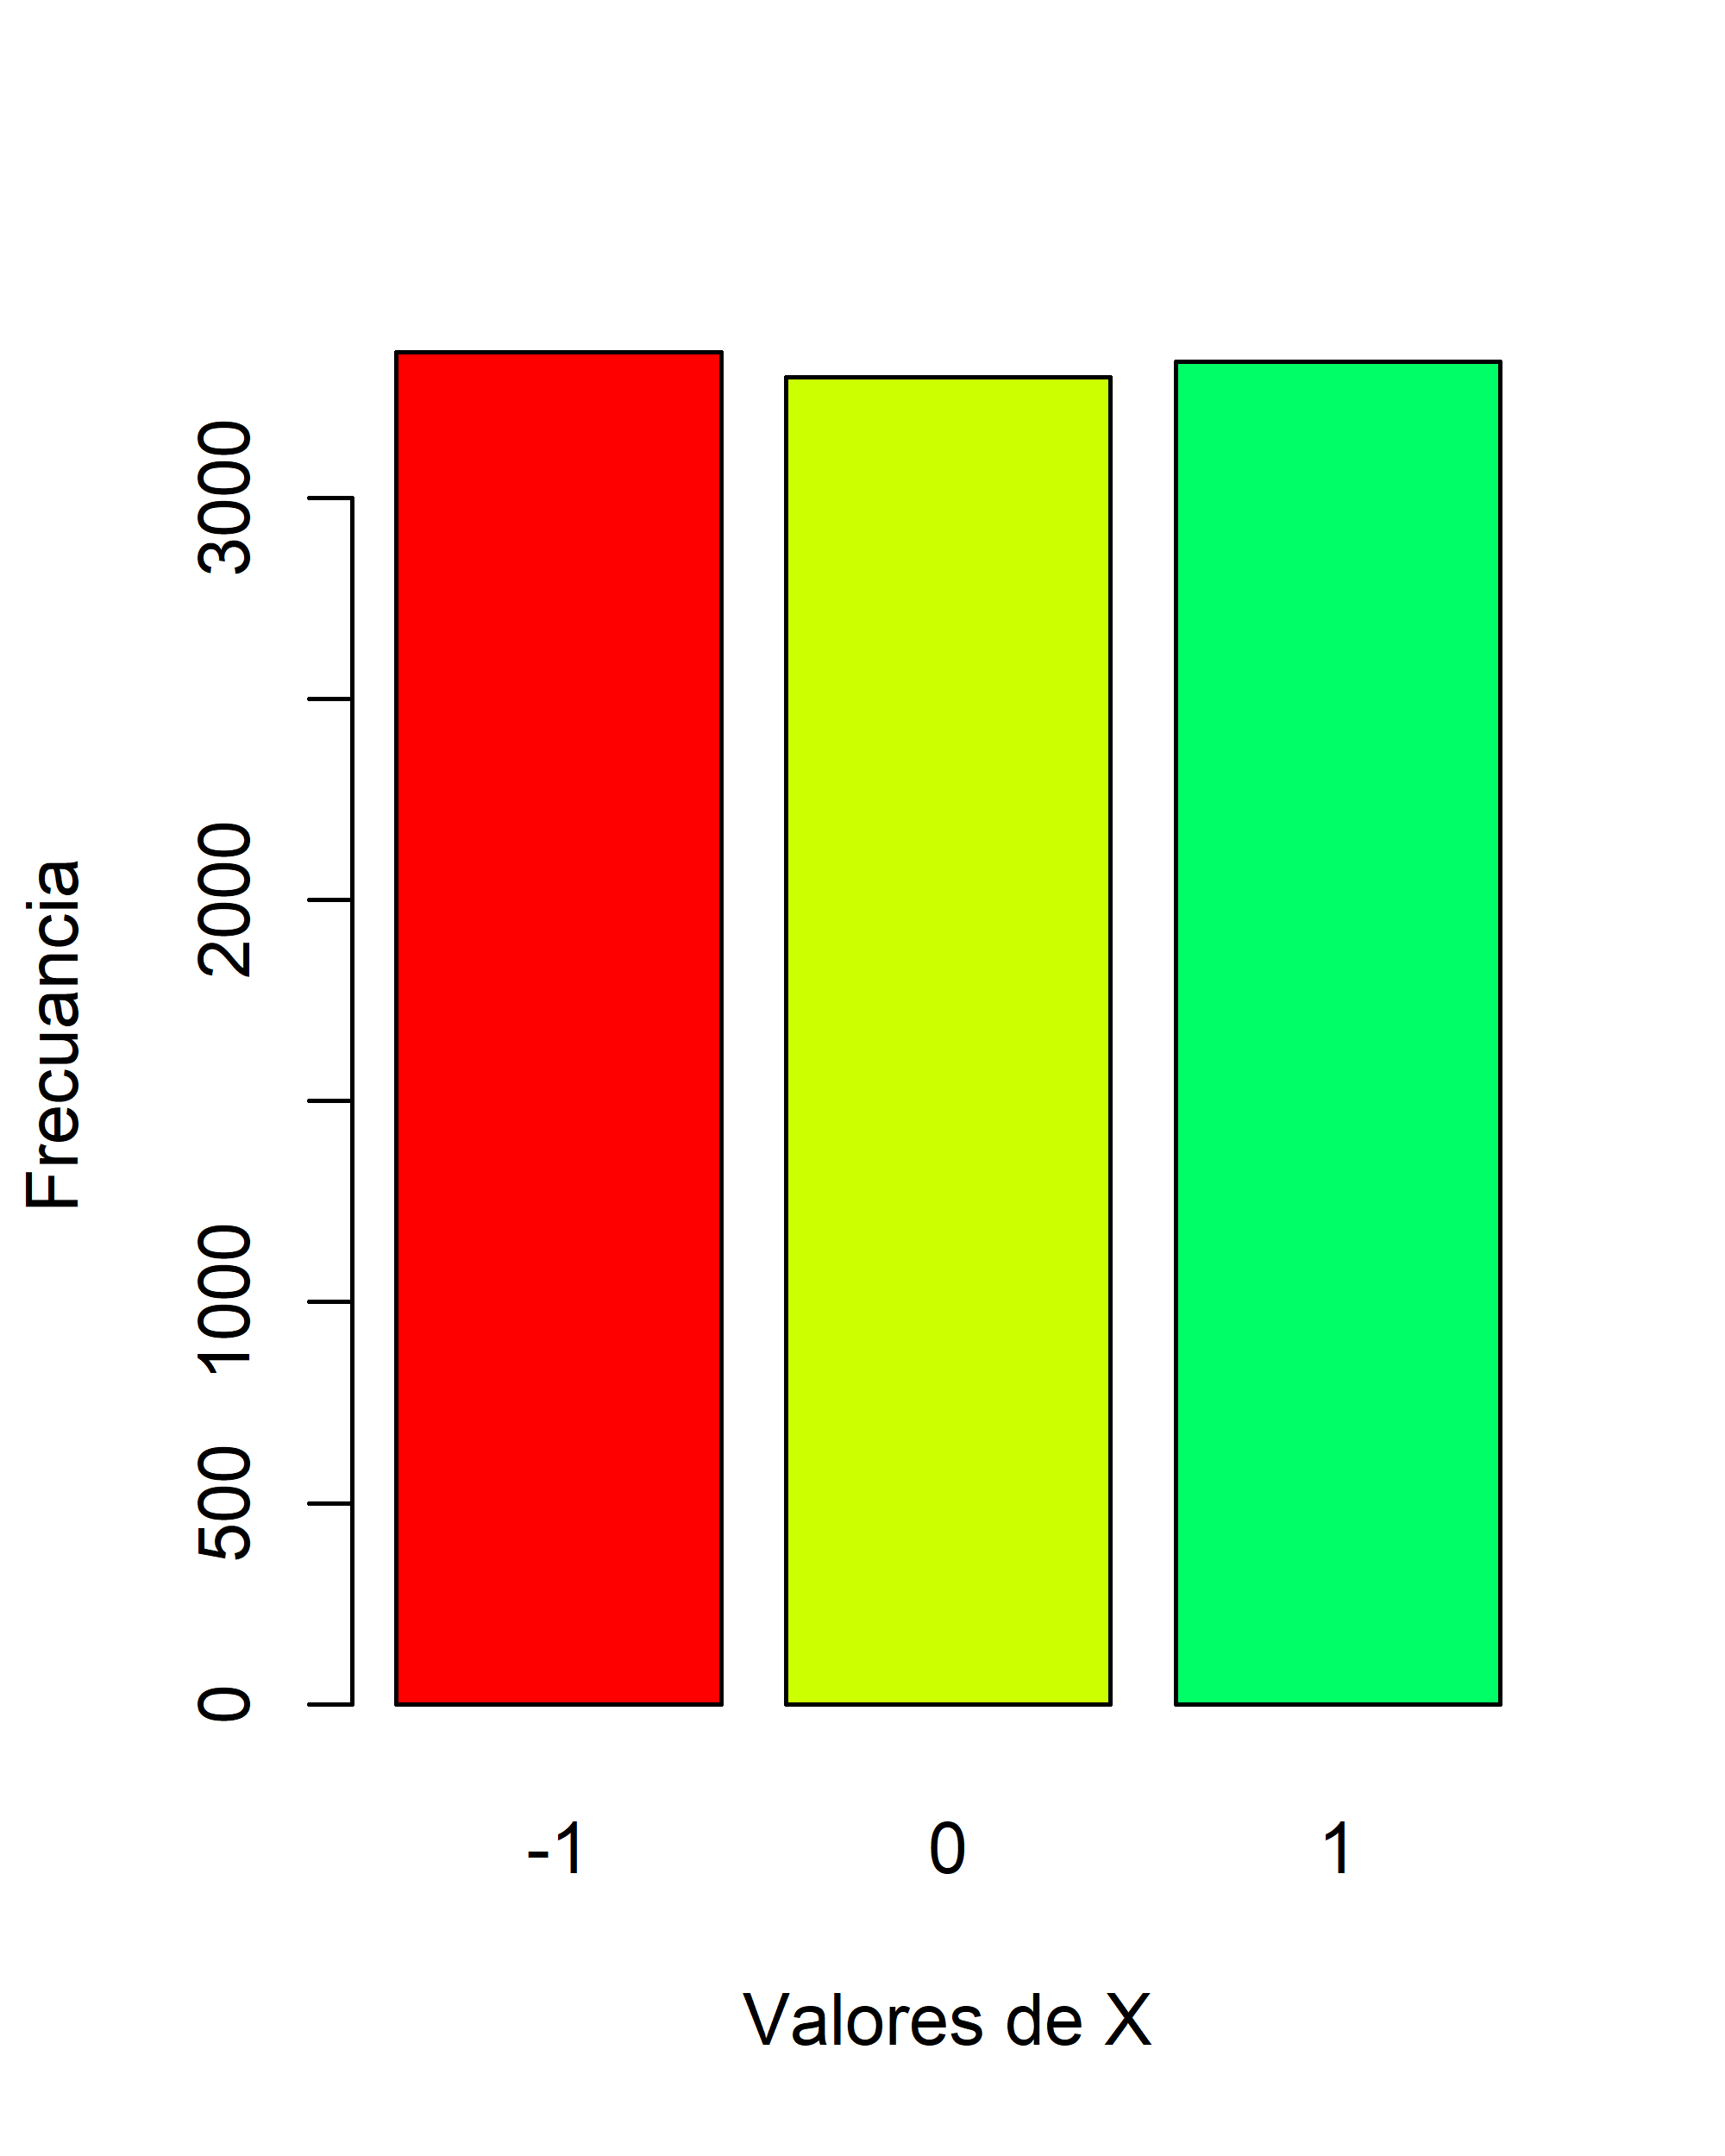
\includegraphics[scale=0.7]{Figures/seleccion.png}
    \caption{Frecuencia de selección entre los números $-1$, $0$ y $1$ (problema \ref{problema4})}
    \label{seleccion}
\end{figure}

\subsection{Problema $3$, página $278$} \label{problema3}
\textit{The lifetime, measure in hours, of the ACME super light bulb is a random variable T with density function $f_{T}(t)$ = $\lambda^2 te^{- \lambda t}$, where $\lambda$ = $0.05$. What is the expected lifetime of this light bulb? What is its variance?}

\noindent \textbf{Solución}

El valor esperado y varianza de la vida útil de las bombillas ACME se calcularon mediante la ecuación \ref{continua} y \ref{varianza}, las cuales arrojaron un $E{(X)}$ = $40$ y una $V{(X)}$ = $2.400$. Se utilizó la función \texttt{integrate()} para realizar estos cálculos.

Para este ejercicio, se realizó una simulación para determinar si el valor esperado y varianza de la vida útil de un lote de $100$ bombillas que siguen una determinada distribución y con función de densidad $f_{T}(t)$ descrita en el problema \ref{problema3}, son iguales o similares a los valores calculados anteriormente. Los resultados de esta experimentación son mostrados en la figura \ref{bombillas}. 

\begin{figure}[h]
    \begin{center}
    \captionsetup{justification=centering}
    \begin{subfigure}[b]{0.45\textwidth}
        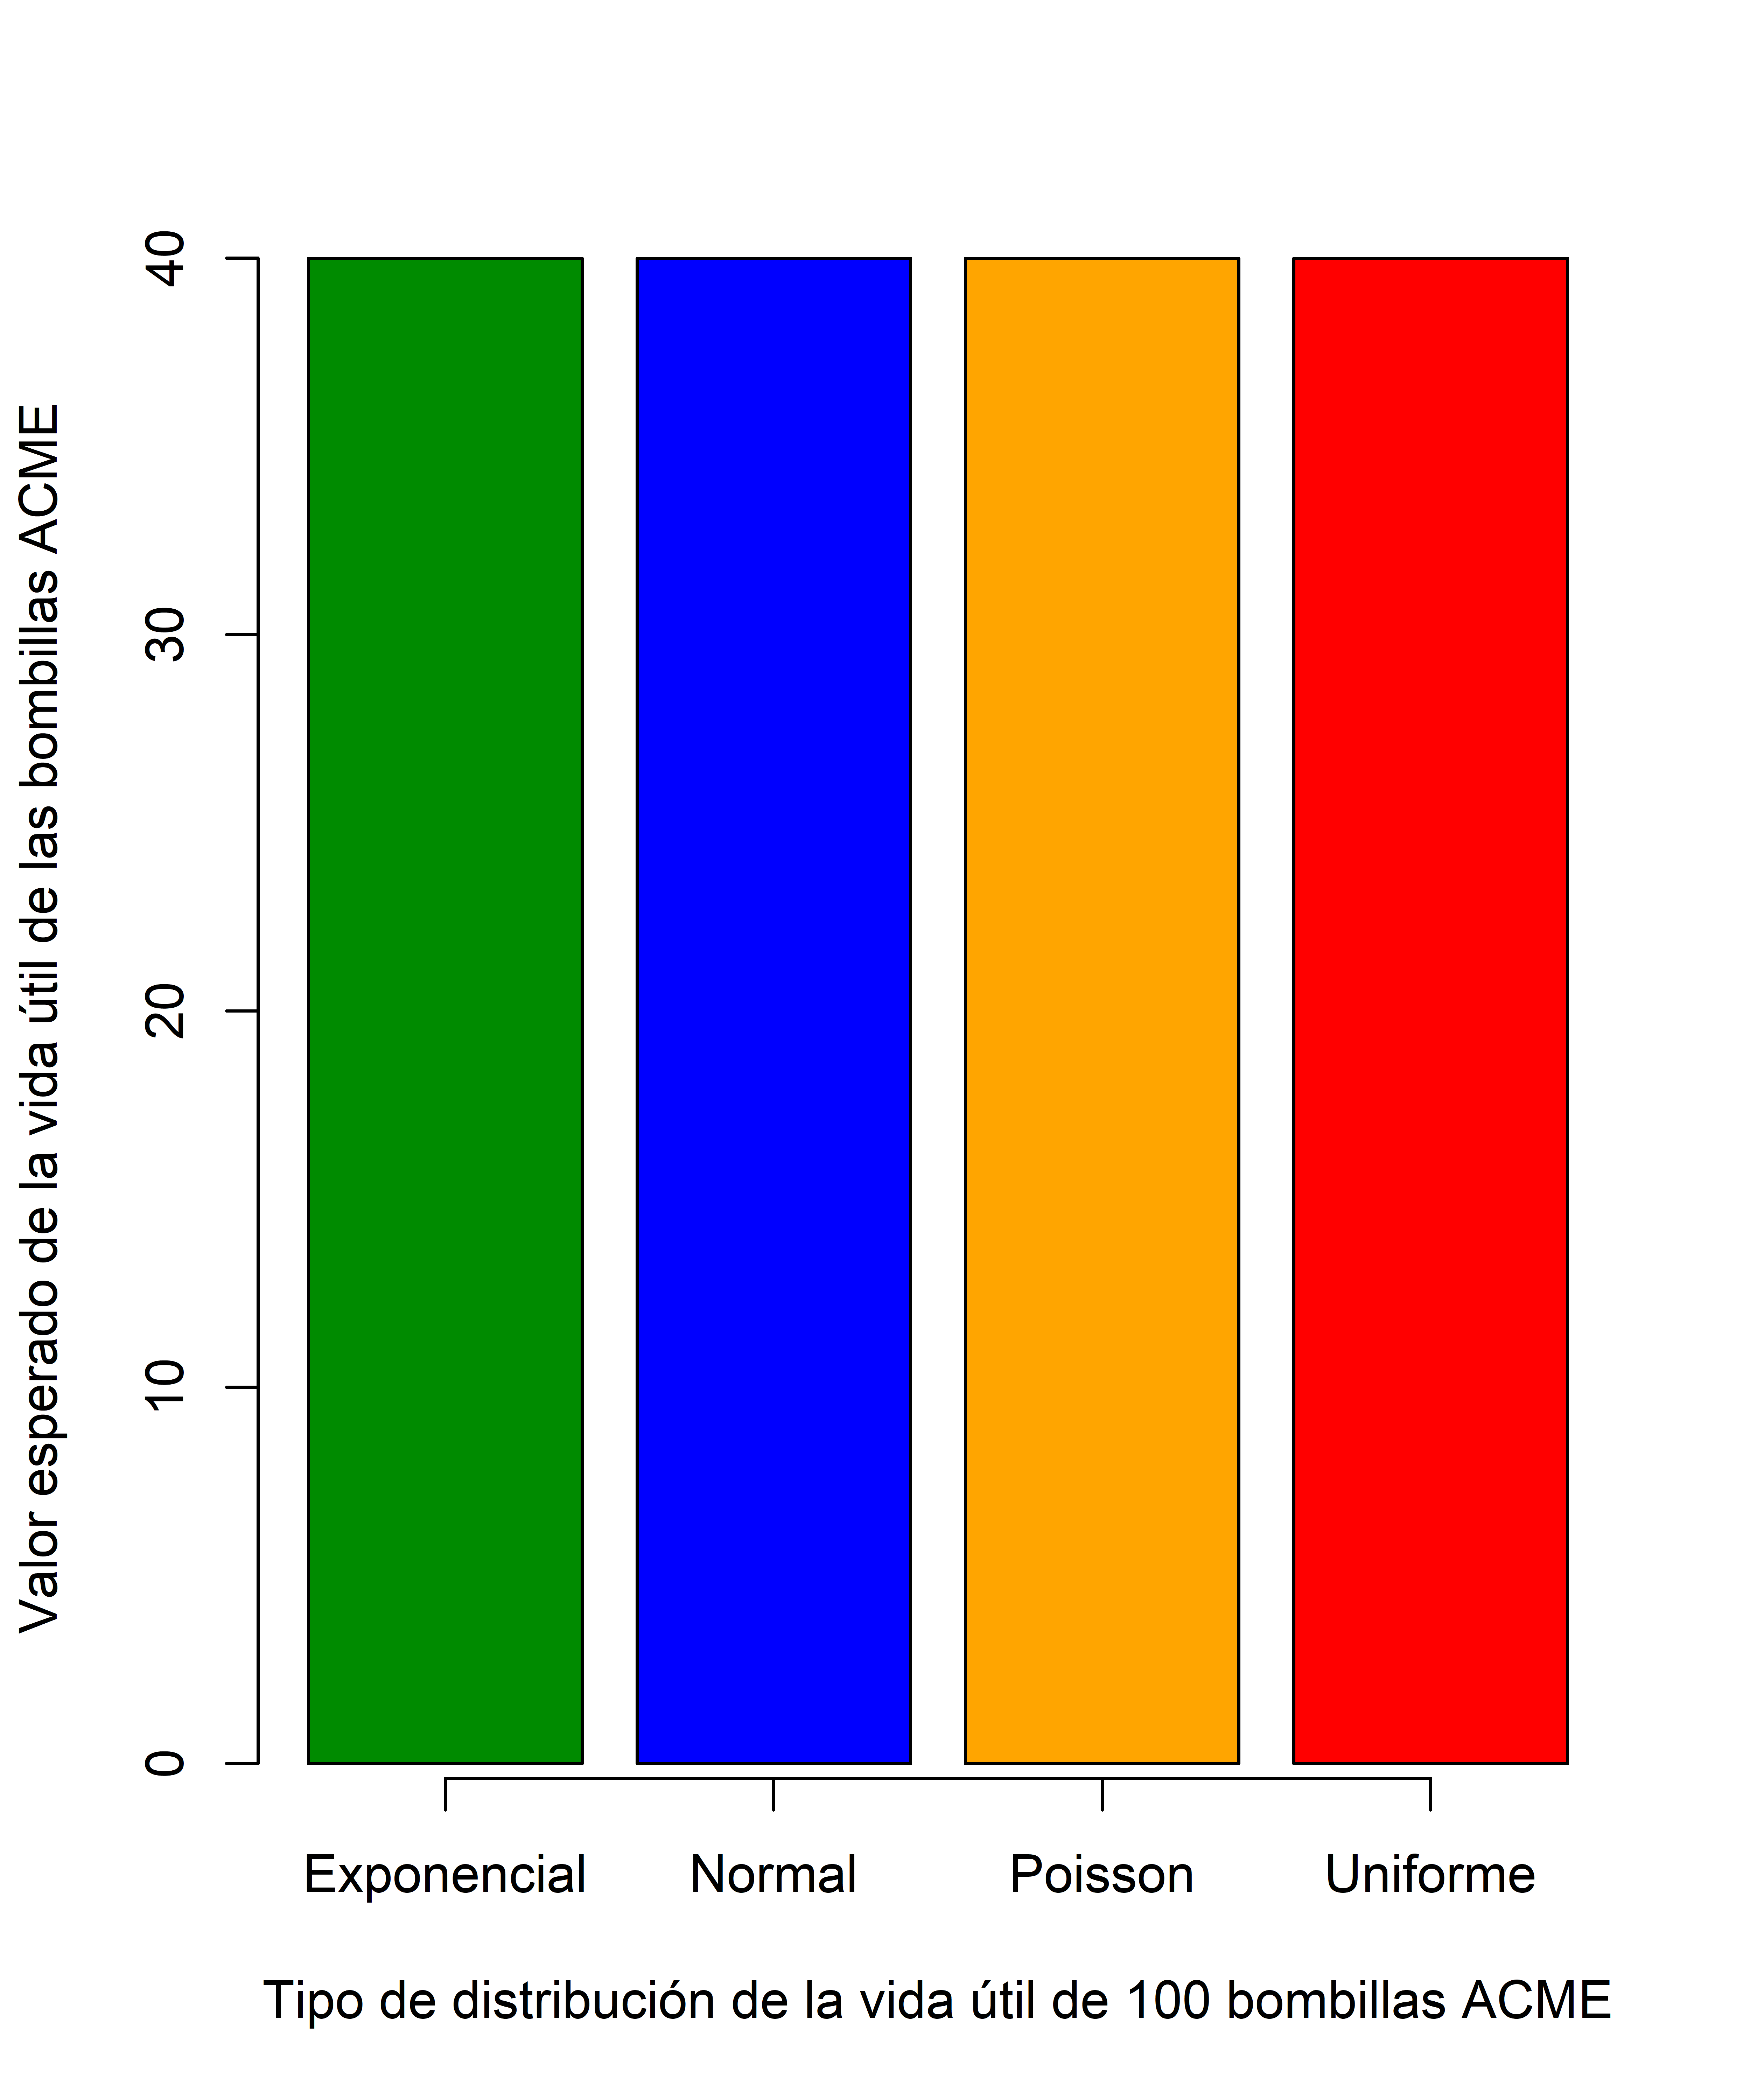
\includegraphics[scale=0.5]{Figures/VEBombillas.png}
        \caption{Valor esperado de las bombillas ACME}
        \label{bombillasVE}
    \end{subfigure}
    \begin{subfigure}[b]{0.5\textwidth}
        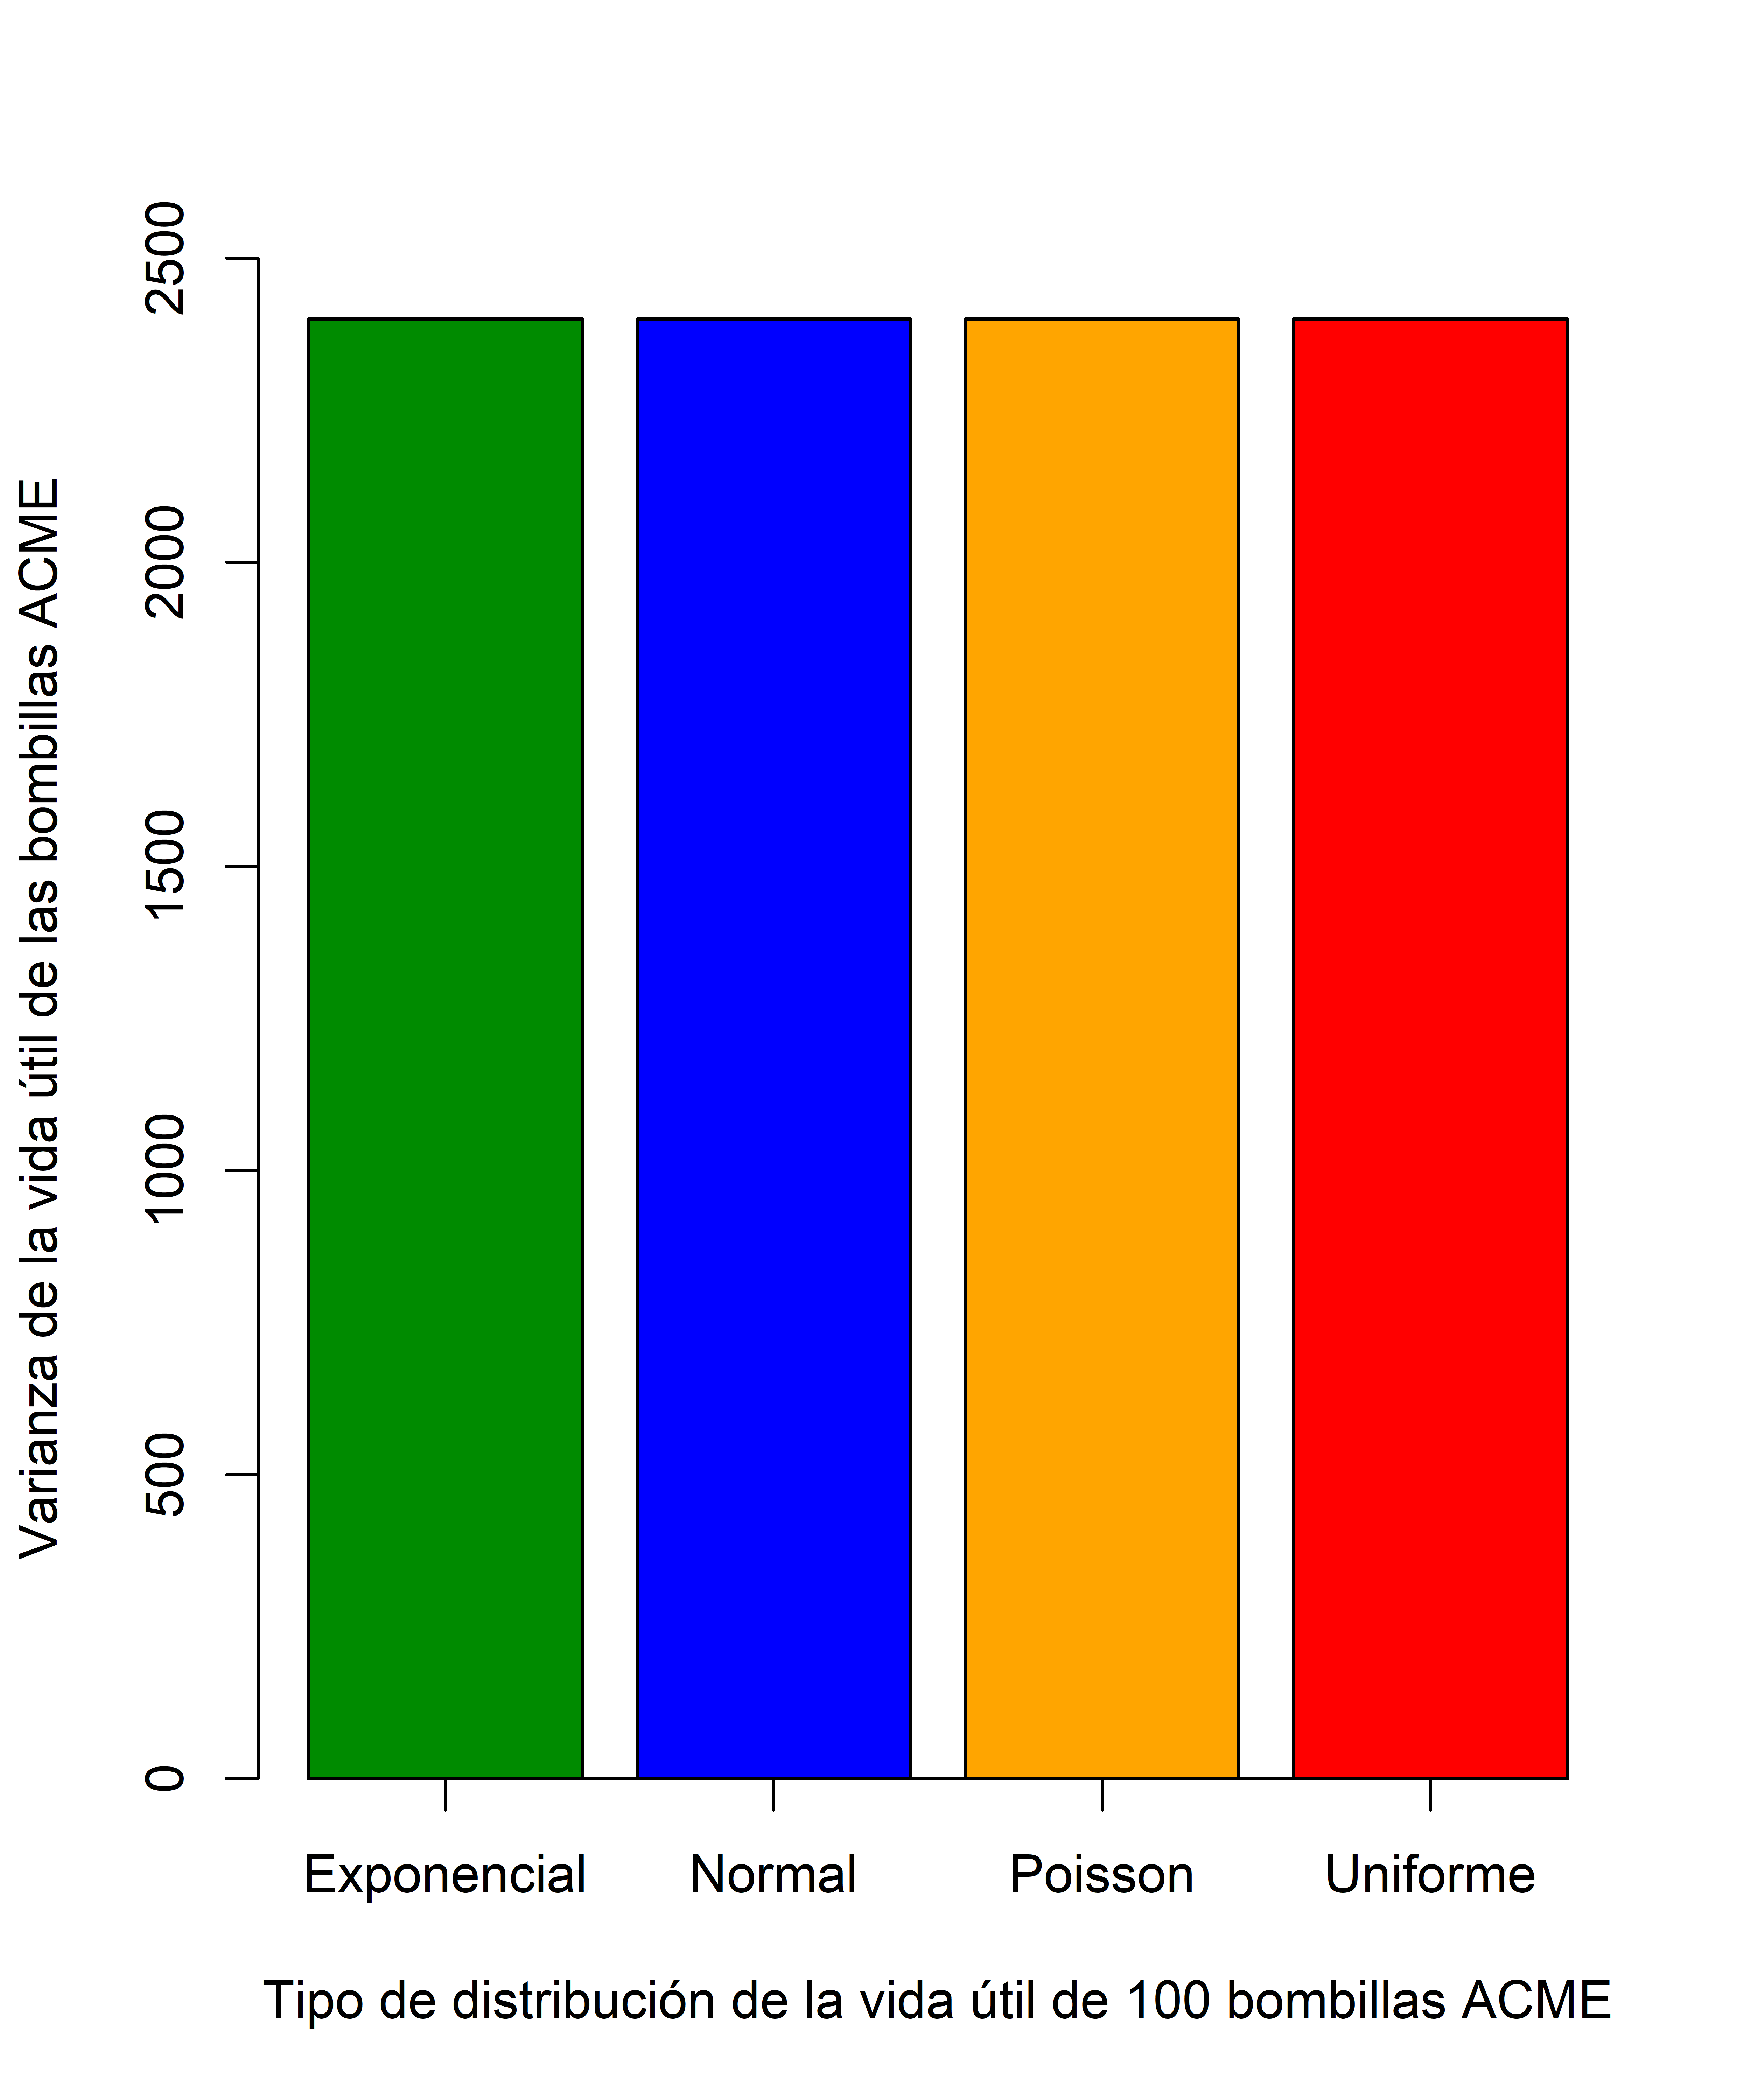
\includegraphics[scale=0.5]{Figures/VarBombillas.png}
        \caption{Varianza de las bombillas ACME}
        \label{bombillasVar}
    \end{subfigure}
    \caption{Resultados simulación para el problema \ref{problema3}}
    \label{bombillas}
    \end{center}
\end{figure}

De acuerdo a lo anterior, podemos observar que en la figura \ref{bombillasVE} y \ref{bombillasVar}, sin importar el tipo de distribución que sigue la vida útil del lote de $100$ bombillas ACME (en este caso, una distribución exponencial, uniforme, normal y de Poisson con valores positivos) el valor esperado y varianza, respectivamente, de la vida útil de estas bombillas es igual al calculado analíticamente, es decir $E{(X)}$ = $40$ y su $V{X()}$ = $2.400$.


\bibliography{refProbabilidad}
\bibliographystyle{plain}

\end{document}
